% ---- ETD Document Class and Useful Packages ---- %
\documentclass{ucetd}
\usepackage{subfigure,epsfig,amsfonts}
\usepackage[round]{natbib}
\usepackage{amsmath}
\usepackage{amssymb}
\usepackage{amsthm}
\usepackage[T1]{fontenc}
\usepackage{multirow}
\usepackage{booktabs}
\usepackage{siunitx}
\sisetup{group-separator={,}, group-four-digits = true}
\usepackage{makecell}
\usepackage{natbib}
\usepackage{minted}
\frenchspacing

%% Use these commands to set biographic information for the title page:
\title{Constraining Mars obliquity history in the Amazonian\\and Hesperian periods using elliptic crater orientations}
\author{James Yunzhang Hu}
\adviser{Edwin S. Kite}
\reader{Dorian S. Abbot}
\department{Geophysical Sciences}
\division{The College}
\degree{Bachelor of Science with Honors}
\date{May 2022}

%% Use these commands to set a dedication and epigraph text
\dedication{\textit{To} waipo}
% \epigraph{Epigraph Text}

\usepackage[pdfusetitle]{hyperref}
\hypersetup{unicode=true,
            linktoc=all,
            pdfsubject=subject here,
            pdfkeywords=keyword1 keyword2 keyword3,
            pdfborder={0 0 0},
            breaklinks=true}
% See https://github.com/k4rtik/ucetd-latex/issues/1
\makeatletter
\let\ORG@hyper@linkstart\hyper@linkstart
\protected\def\hyper@linkstart#1#2{%
  \lowercase{\ORG@hyper@linkstart{#1}{#2}}}
\makeatother

\begin{document}
%% Basic setup commands
% If you don't want a title page comment out the next line and uncomment the line after it:
\maketitle
%\omittitle

% These lines can be commented out to disable the copyright/dedication/epigraph pages
% \makecopyright
\makededication
% \makeepigraph


%% Make the various tables of contents
\tableofcontents
\listoffigures
\listoftables

\acknowledgments
I would like to thank my adviser Edwin Kite, without whom this project would not be possible, for his ideas, knowledge, guidance, and direction throughout this yearlong endeavor during which I have learned so much about Mars and planetary science. I’m also grateful to Dorian Abbot for his constructive comments and insights.

I’d also like to thank my program instructors and colleagues at the Marine Biological Laboratory in Woods Hole for condoning mid-lecture crater-tracing (and for giving me a great first taste of original scientific research). Thanks especially to Alice Ball for our thesis focus sessions.

Thank you to mum and dad for buying every space and dinosaur encyclopedia little me ever wanted and, more recently, listening to me ramble about \citet{holo2018a}. Thank you to my dearly missed \textit{waipo}, to whom this thesis is dedicated. Thank you to Puyu Shi for her constant love and support.

\abstract
Mars’s past obliquity governs many aspects of its past climate, including its surface volatile dynamics, atmospheric collapse, and low-latitude ice migration. Yet because Mars obliquity oscillates chaotically over >100~Ma time scales, the bulk of Mars’s past obliquity cannot be determined through physical simulations and is therefore unknown. This study attempts to constrain Mars’s past obliquity by adapting a recently developed statistical technique that compares the orientations (azimuths) of actually observed elliptic craters to those of simulated craters under different obliquity scenarios in which Mars obliquity was held constant over the simulated time period. To obtain the azimuths of actually observed elliptic craters, we traced 1,678 elliptic craters collectively from the late Amazonian volcanic (lAv) and Amazonian--Hesperian volcanic (AHv); separately, we simulated $10^6$ craters per constant-obliquity scenario for each geologic unit. We compared then the actual and simulated craters’ respective azimuth distributions with the azimuth distributions, measuring the extent of simulation--data mismatch by conducting $\chi^2$ tests whereby the best-fit obliquity scenarios were those yielding the smallest reduced $\chi^2$ statistic, for each geologic unit. We found that the mean obliquities associated with the lAv unit, representing the past $\sim$0.9~Ga, and AHv unit, representing the past $\sim$2.0~Ga, were 66° (56.2°--74.6° standard deviation interval) and 8° (0.0°--14.4° standard deviation interval), respectively. As a sensitivity test, we quantified the inter-analyst tracing error on azimuth measurements and applied those errors at random to our crater azimuths 1,000 times, thus generating 1,000 new sets of 1,678 inter-analyst-perturbed crater azimuths. We found (in our median inter-analyst-perturbed result) that the mean obliquities associated with the lAv and AHv units were 63° (54.7°--72.0° standard deviation interval) and 14° (6.3°--20.5° standard deviation interval), respectively. These results’ geologic implications include that, relative to today ($\sim$25° obliquity), Mars saw, over the past $\sim$2.0~Ga, more intense polar glaciation, polar atmospheric collapse, and desiccation of deep aquifers and saw, over the past $\sim$0.9~Ga, greater sublimation of water ice, the migration to lower latitudes of water ice, higher water vapor pressure, and more frequent polar dust storms. Future work may collect a larger set of craters, apply this study’s methods to \citet{holo2018a}’s dataset and vice versa, account for poke-throughs of older craters on younger terrain, and investigate why our method implies an unphysical result for the intervening $\sim$1.0~Ga period between the ages of the units.
\mainmatter
% Main body of text follows

\chapter{Introduction}
\label{chapter:1}

\section{Theoretical background on Mars obliquity variation}
\label{section:1-1}

Currently at $\sim$25°, Mars obliquity, or the tilt of its polar axis relative to the normal to its orbital plane, has varied dramatically over geologic time, primarily because of gravitational forcing by Jupiter \citep{laskar2004a}. The obliquity evolution of post-Noachian Mars is of great interest as it has strongly affected its climate, atmosphere, hydrology, and surface features; accurate reconstructions of Mars obliquity history are critical to the study of the planet’s paleoclimates and past habitability \citep{ward1973a, jakosky1985a, laskar2004a}.

Through the reverse integration of Mars’s orbital and rotational equations, reconstruction efforts have identified significant obliquity variations on both periodic and secular timescales \citep{ward1973a, touma1993a, laskar1993a, laskar2004a}. The obliquity of Mars presently oscillates between $\sim$15° and $\sim$35° within periods of $\sim$100~ka--1~Ma (in stark contrast to Earth’s Moon-stabilized obliquity, which stays within ±1.3° of the mean value), although over the past $\sim$300~ka the amplitude has temporarily decreased to just a few degrees from the mean \citep{laskar2004a}. The past obliquity of Mars is precisely characterized to $\sim$20~Ma ago, when it oscillated around a mean of $\sim$35° before abruptly transitioning to the present range at $\sim$5~Ma ago \citep{laskar2004a, laskar2010a}.

Beyond $\sim$100~Ma ago, however, chaotic diffusion dominates, because the moments of inertia of Mars can change such that the planet encounters secular spin-orbit resonances---events wherein the period of spin axis precession matches a period in the variation of Mars’s orbital plane inclination---that, in turn, cause large, unpredictable swings in obliquity \citep{ward1979b}. Consequently, obliquity may have wandered between 0° and $\sim$70°, such that the bulk of Mars obliquity history since Solar System formation cannot be exactly recovered through numerical integration \citep{touma1993a, laskar1993a, laskar2004a}. To characterize Mars obliquity history beyond the geologically recent past, today’s researchers have therefore been forced to eschew numerical integration in favor of statistical analysis and surface observation \citep[e.g.,][]{laskar2004a, holo2018a}.

\section{A brief history of Mars obliquity reconstruction}
\label{section:1-2}

As summarized by \citet{laskar2004a}, Mars researchers initially placed their focus on the precession of the planet’s axis and the evolution of its eccentricity \citep{leighton1966a, murray1973a}. Applying the same lens as those who pointed out that Earth’s ±1.3° oscillations in obliquity have significantly shaped its paleoclimate, \citet{ward1973a} calculated that Mars had experienced ±$\sim$10° oscillations and concluding that resolving past obliquity forcing would be indispensable to the understanding of features including its paleoclimate, paleohydrology, and surface geology. In parallel, advancements in computing technology, astronomical calculation, and space exploration successively improved researchers’ ability to constrain the recent (past $\sim$100~Ma) obliquity history of Mars \citep[e.g.,][]{brouwer1950a, bretagnon1974a, laskar1988a, folkner1997a, yoder1997a}.

By far the most significant advancements in the understanding of Mars obliquity variation, however, have not been the refinement of deterministic reverse integrations. It was originally thought that, even on $\sim$1~Ga timescales, obliquity non-chaotically oscillated around $\sim$25° in the post-Noachian period \citep{ward1974a, ward1979a, ward1992a}. Separately by \citet{touma1993a} and by \citet{laskar1993a}, it was proposed that chaotic secular spin-orbit resonances pose an insurmountable barrier to the numerical solution of >100~Ma ago Mars obliquity. \citet{laskar2004a} later reinforced this result by statistically demonstrating that, based on a large number of obliquity solutions and orbital solutions, chaotic diffusion dominates the planet’s obliquity evolution over secular timescales. \citet{bills2019a} posited, in dissent, that obliquity variations are likely non-chaotic because small magnitudes of energy dissipation can dampen chaotic variations, and moreover that obliquity variations are fully damped such that future variations can be computed; yet even they agree that past obliquity oscillations (except the past mean obliquity) cannot be accessed.

\section{Relevance and indirect evidence of Mars obliquity variation}
\label{section:1-3}

Past obliquity oscillations are particularly relevant to the history of surface volatiles, especially water and CO\textsubscript{2}, on Mars \citep[reviewed in][]{jakosky2021a}. A primary mechanism through which obliquity modifies Martian climate is by controlling the summer insolation on polar ice caps, which are composed of both water ice and dry (CO\textsubscript{2}) ice. Whereas the poles are well shielded from the Sun at low obliquity, they experience intense summer insolation at high obliquity. In the former case, colder poles thin out the atmosphere by precipitating gaseous CO\textsubscript{2}, thus driving the collapse of the Martian atmosphere at the poles \citep{lindner1985a, kreslavsky2005a, phillips2011a, soto2015a}. In the latter case, polar water ice undergoes enhanced sublimation, both migrating to lower latitudes and increasing the pressure of water vapor \citep{haberle1990a, jakosky1995a, zent2013a, forget2017a}. Further consequences of dramatic obliquity excursions relate to dust storms, more likely to initiate near poles at high obliquity, and deep aquifers, more likely to desiccate via sublimation at low obliquity \citep{haberle2003a, grimm2017a}.

Indirect evidence of past obliquity oscillation is present in various forms. Although water ice is presently unstable below polar latitudes on present-day Mars, there exists extensive evidence of mid- and low-latitude debris-covered glaciers, which likely formed due to the migration of polar ice in periods of high obliquity \citep{head2003b, dickson2008a, adeli2019a}. Geomorphic features like mid-latitude smooth mantled deposits and glacial deposits on the northwestern flanks of Tharsis Montes further suggest water ice was deposited below polar latitudes, likely during high obliquity \citep{mustard2001a, head2003a, head2003b, milkovich2006a,  shean2007a}. The formation of mid-latitude and tropical glaciers during past ice ages were also likely significantly controlled by high-obliquity excursions, and such ice ages may have accounted for one-quarter of the post-Noachian period  \citep{forget2006a, madeleine2009a, weiss2019a}. The rates of deposition and ages of polar layered deposits of CO\textsubscript{2} also depend critically on large-scale obliquity oscillations \citep{manning2019a, emmett2020a}.

\section{Geologic constraints on historical Mars obliquity}
\label{section:1-4}

\citet{holo2018a} devised a statistical-computational pipeline to constrain the post-Noachian obliquity of Mars that exploited evidence imprinted by grazing bolide impacts upon geologic units of known age. When impactors strike Mars at a low angle of incidence, they create craters that are elliptic and hence oriented. In aggregate, the orientations of such elliptic craters can inform us of the past obliquity of Mars; in particular, the overall distribution of elliptic crater azimuths (orientations from due north) on Mars depends on obliquity such that, at low obliquity, craters are more north-south oriented (low azimuth) and, at high obliquity, they tend to be more east-west oriented (high azimuth). (The mechanics of this process are explained further in §\ref{section:2-3}.) Taking the azimuths of elliptic craters from the Robbins global Mars crater database \citep{robbins2012a}, \citeauthor{holo2018a} compared the real azimuth distribution to predicted azimuth distributions of craters generated by causing randomly seeded impactors to strike Mars, whose obliquity at the time of impact was determined by a simulated obliquity history; each prediction of azimuth distribution thus corresponded to a different simulated Mars obliquity history \cite{kite2015a}. Assigning a heavier weighting to the histories whose predicted azimuth distributions best matched that of the actual geologic data, \citeauthor{holo2018a} then calculated the weighted-average probability density function for the mean obliquity and fraction of time with obliquity >40°.

\citet{holo2018a} concluded that, during the Hesperian, Mars’s mean obliquity was likely between $\sim$10° and $\sim$30° (lower than the unweighted prior, i.e., the mean obliquity calculated by equally weighting all of the simulated Mars obliquity histories) and rejected at the 95~percent confidence level that mean obliquity was $\gtrsim$33°. To produce this result, they assumed that their simulated impactors were representative of post-Noachian Mars history and were not biased in terms of inclination; that the size frequency distribution of their impactors was representative of those that have struck post-Noachian Mars; that the 1,502 craters they studied were a representative sample of all elliptic post-Noachian craters; and that geologic surface processes and crater collapse did not excessively deform crater morphologies so as to obscure crater azimuths at the time of formation. While their study produced an overall prediction of late Hesperian--onward obliquity, they could not distinguish between mirrored obliquity histories (i.e., those that start low and end high and those that start high and end low) and could not comment on Amazonian-specific Mars obliquity history. Their methodology is also difficult to apply to even earlier periods in Mars history due to the heavy degradation of craters on Noachian geologic units.

As \citet{holo2018a} pointed out, there have been few attempts to geologically constrain Mars obliquity history; relevant studies have been Earth-based and indirect or tangential. For example, \citet{ma2017a} demonstrated using an astronomical clock, developed by \citet{sageman2014a} using stratigraphic evidence from the Cretaceous Western Interior Basin, that Mars--Earth resonance transitions are chaotic, while \citet{kent2018a} used a magnetic polarity sequence from Earth to confirm the stability of the 450~ka Jupiter--Venus eccentricity cycle. Relatedly, \citet{olsen2019a} used the Geological Orrery, a systematic record of Triassic and Jurassic lake sediment deposits temporally correlated to changes in Earth's orbital properties, to recover values for the precessions of the perihelion for Mercury, Venus, Earth, and Mars, while \citet{mau2022a} found evidence of long-term climate cycles on Earth, attributed to Earth--Mars gravitational intersections, using chronostratigraphic records. These studies offer insight into how future researchers might marshal Martian geologic evidence for the study of planetary orbital properties by emulating methods used on Earth samples, but they do not directly investigate Mars obliquity history. At present, the statistical analysis of elliptic crater orientations and dating of ice deposits seem to be the only feasible ways to geologically constrain Mars obliquity.

\section{Overview of this study}
\label{section:1-5}

This study attempts to constrain the mean obliquity of Mars over two time periods: $\sim$0.9~Ga ago to present and $\sim$2.0~Ga ago to present. We adapt \citet{holo2018a}’s forward model (i.e., its algorithm for generating predicted obliquity-specific azimuth distributions) to a new dataset consisting of craters in the Amazonian and Amazonian-Hesperian volcanic units. In §\ref{chapter:2}, we detail the data collection process (§\ref{section:2-2}), modifications to and use of \citet{holo2018a}’s forward model (§\ref{section:2-3}), statistical comparison of simulated and observed crater azimuth probability distribution functions and determination of the ages of Martian geologic units (§\ref{section:2-4}), and sensitivity checks (§\ref{section:2-5}). In §\ref{chapter:3}, we present our results: the simulated and observed azimuth probability distributions (§\ref{section:3-1}), the mismatch between simulated and observed azimuth probability distributions as a function of obliquity (§\ref{section:3-2}), and the reconstructed mean obliquity of Mars over absolute geologic time (§\ref{section:3-3}). In §\ref{chapter:4}, we first discuss the overall trends in the results (§\ref{section:4-1}), compare our results to those in the literature (§\ref{section:4-2}), perform sensitivity tests (§\ref{section:4-3}), discuss the implications of our results for past Martian climate and hydrology (§\ref{section:4-4}), and discuss the limitations of this study (§\ref{section:4-5}). We conclude in §\ref{chapter:5}.

\chapter{Methods}
\label{chapter:2}

\section{Overview of methods}
\label{section:2-1}

This study’s methods are summarized in Figure~\ref{fig:2-1}. Our procedure comprised four broad stages, of which Stages 1, 2, 3, and 4 respectively correspond with §\ref{section:2-2}, §\ref{section:2-3}, §\ref{section:2-4}, and §\ref{section:2-5}. We used MATLAB version R2022a to perform data analyses and create figures \citep{MATLAB:2022}; translucent lines in figures were drawn using a custom script \citep{shoelson2012a}.

\begin{figure}
    \includegraphics[width=\textwidth]{figures/fig2_1.png}
    \caption[Flow chart overview of this study’s methods]{Flow chart overview of this study’s methods.}
    \label{fig:2-1}
\end{figure}

\section{Collection of crater azimuth data}
\label{section:2-2}

We focused on two units on the surface of Mars, distinguished by their composite morphology, infrared brightness, and thickness, among other factors, according to \citet{tanaka2014a}: the younger late Amazonian volcanic (lAv) unit and a portion of the older Amazonian--Hesperian volcanic (AHv) unit. Note that while the lAv unit is younger than the AHv unit, the former is distinct from and not a subset of the latter; see §\ref{section:2-4} for how each unit was dated based on the age of the underlying rock. The lAv unit stretches from southern Elysium Planitia in the eastern hemisphere to much of Amazonis Planitia in the western hemisphere, and additionally includes Marte Vallis, peripheral areas east of Olympus Mons, and northeastern Ceranius Fossae. The AHv unit encompasses most of the Tharsis and Elysium Rises, as well as part of Amazonis Planitia. As indicated in Figure~\ref{fig:2-2}, we sampled craters in the entirety of the lAv unit and, for the AHv unit, only sampled the NW quadrant, i.e., southern Amazonis Planitia and northern Tharsis Rise.

This study considered craters identified in the Robbins global Mars database of 384,343 Mars craters with diameters of at least 1~km \citet{robbins2012a}. Using JMARS version 5.2 \citep{christensen2009a}, analyst 1 (James Hu) traced the rims of 3,999 craters (all 1,726 craters in the lAv unit, plus 2,273 craters in the AHv unit) using the “Add Points” feature in separate map layers, then exported the traces as shapefiles. We subsequently employed an ellipse-fitting script to convert the shapefiles into ellipses, thus yielding data on the craters’ diameters, center coordinates, ellipticities, and azimuths \citep{gal2003a}. For two example pairs of crater traces and ellipse fits, see Figure~\ref{fig:2-3}. Finally, we filtered the craters for an ellipticity (defined as the length of the major axis over that of the minor axis) >1.05. As shown in Figure \ref{fig:2-4}, most craters have ellipticity <1.05. Including craters that are insufficiently elliptic would risk introducing large errors in crater azimuth, as even small imprecisions in tracing could cause large errors in azimuth. A threshold of 1.05 is the maximum that allows for an overall dataset size at least as large as that in \citet{holo2018a}; a 1.10 threshold, for instance, would only yield 521 craters and 1.15 only 248 (see §\ref{section:4-3} for alternative results should our procedure have set 1.10 or 1.15 as the threshold). This made for a final dataset of 1,678 elliptic craters (761 in the lAv unit and 917 in the AHv unit).

\begin{figure}
    \i
    \includegraphics[width=\textwidth]{figures/fig2_2.jpg}
    \caption[\citet{tanaka2014a} geologic map of Mars, with sampled areas outlined]{\citet{tanaka2014a} geologic map of Mars, with sampled areas outlined: aqua outline: lAv unit; lime outline: surveyed portion of the AHv unit.}
    \label{fig:2-2}
\end{figure}

\begin{figure}
    \centering
    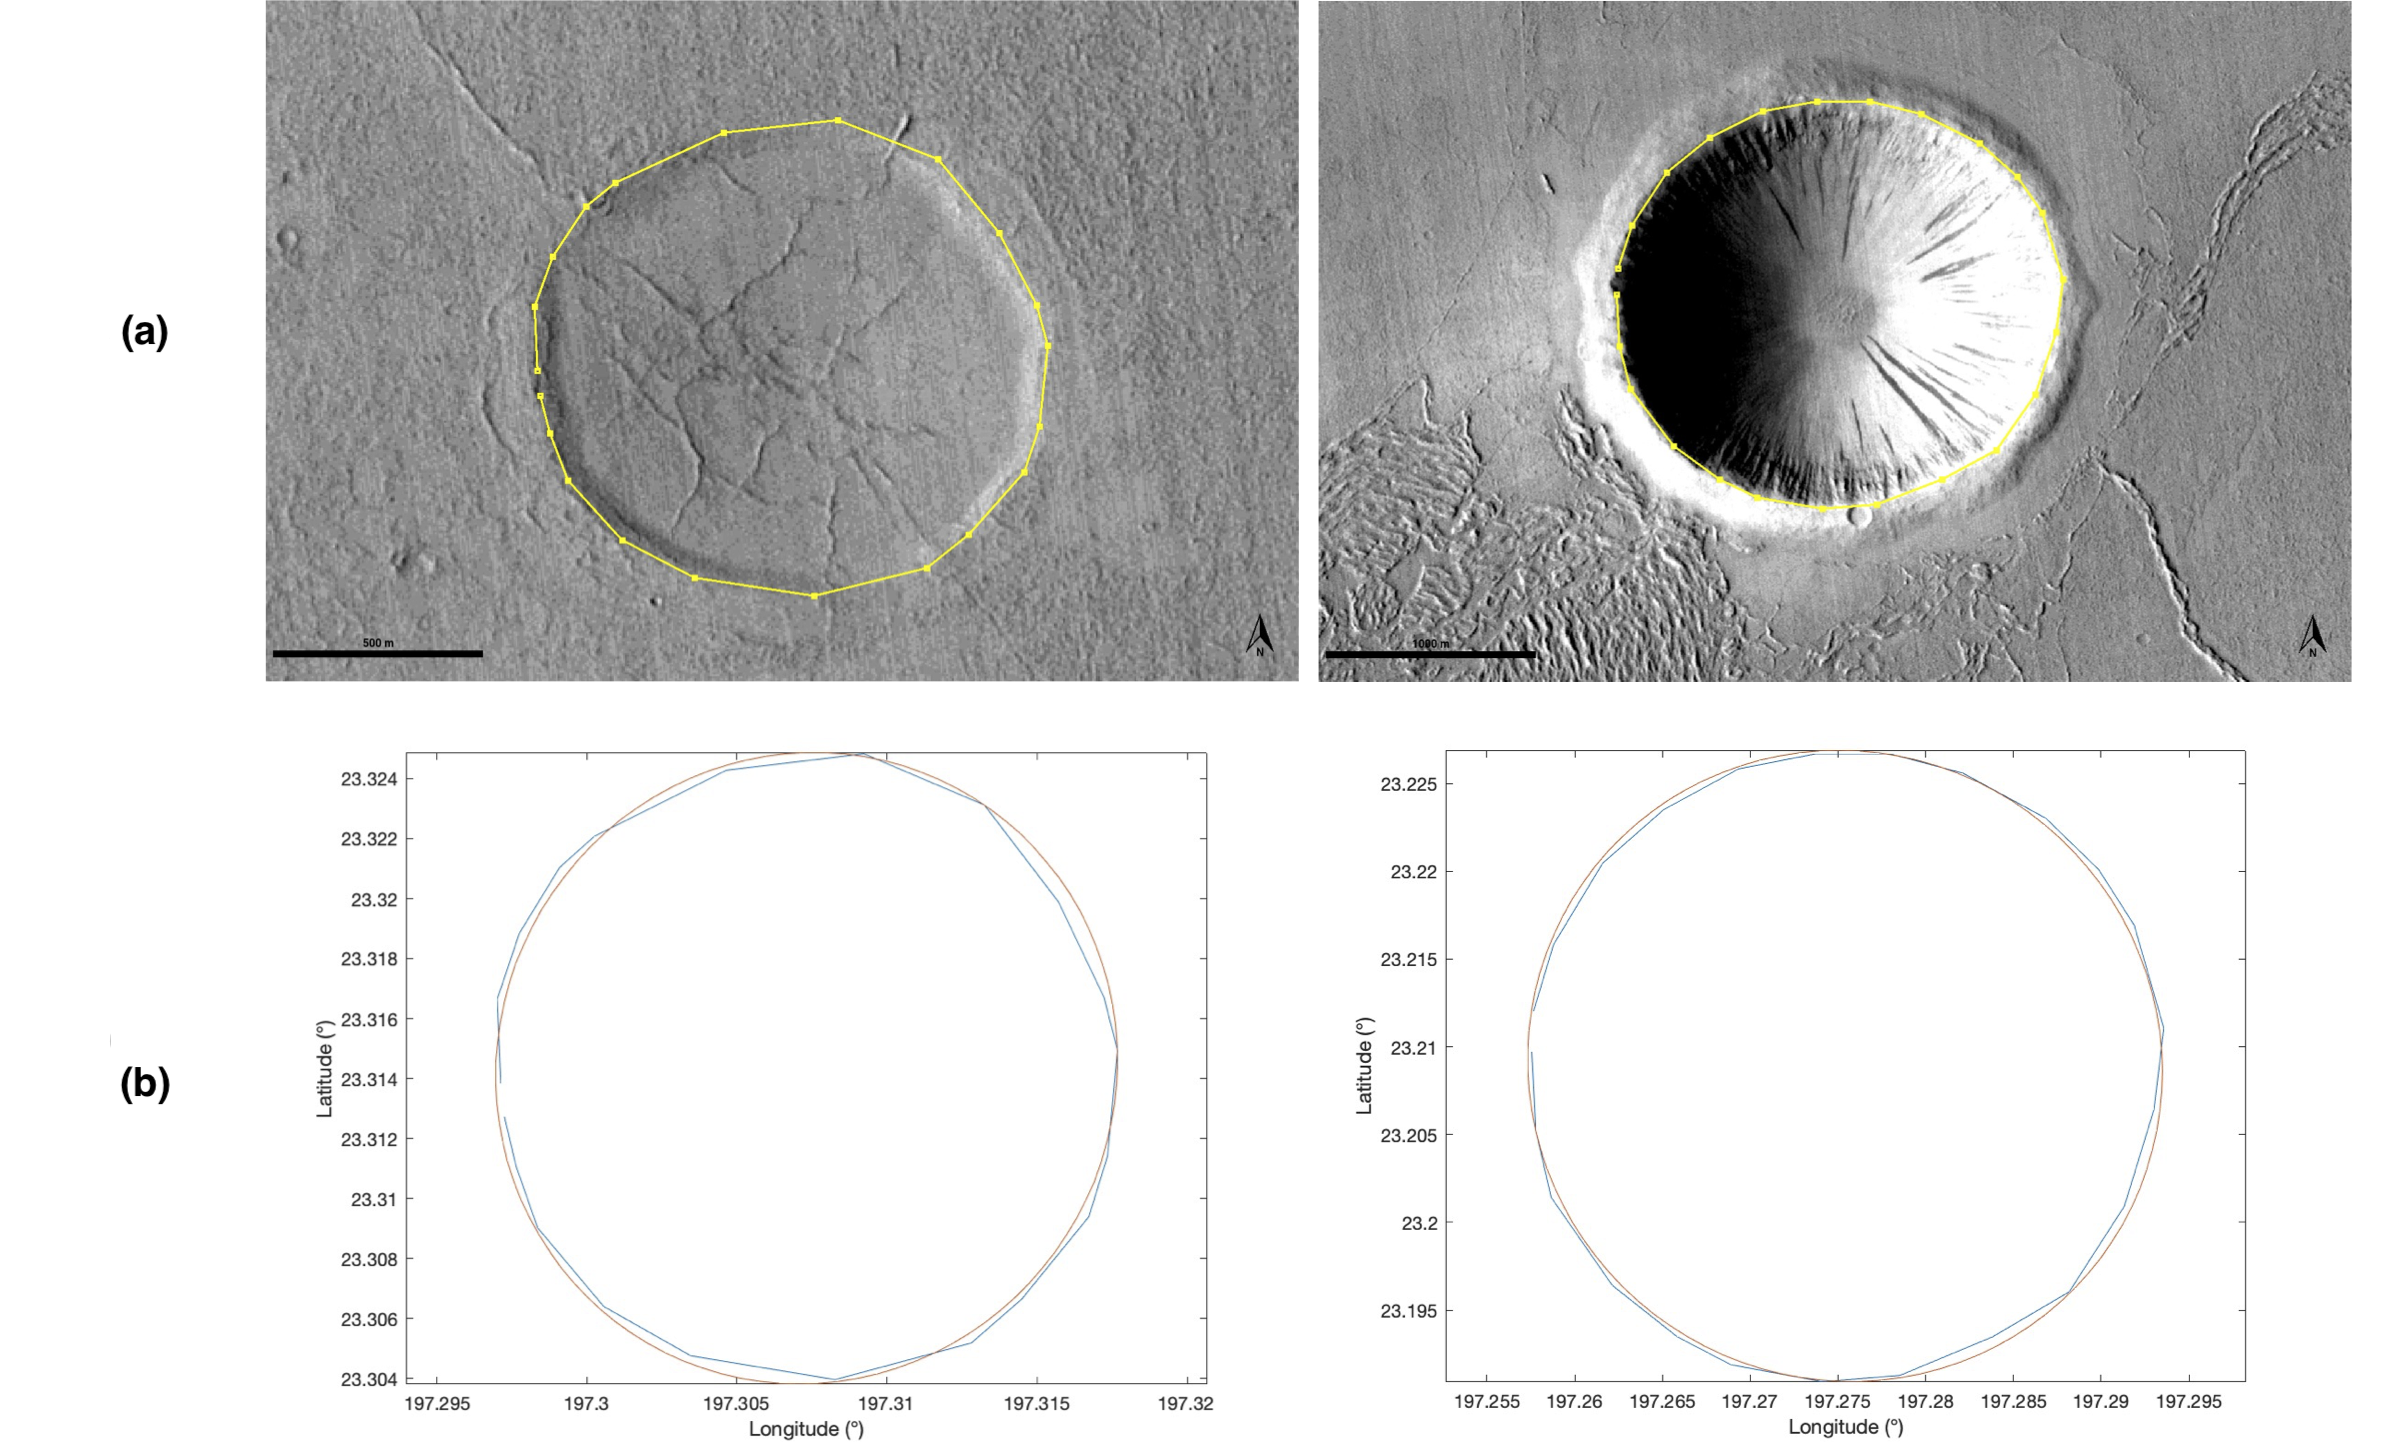
\includegraphics[width=\textwidth]{figures/fig2_3.png}
    \caption[Two sampled craters in the AHv unit]{Two sampled craters in the AHv unit: (a) the crater rims are traced in JMARS 5.2; (b) the traced coordinates (blue) are fitted to smooth ellipses (orange).}
    \label{fig:2-3}
\end{figure}

\begin{figure}
    \centering
    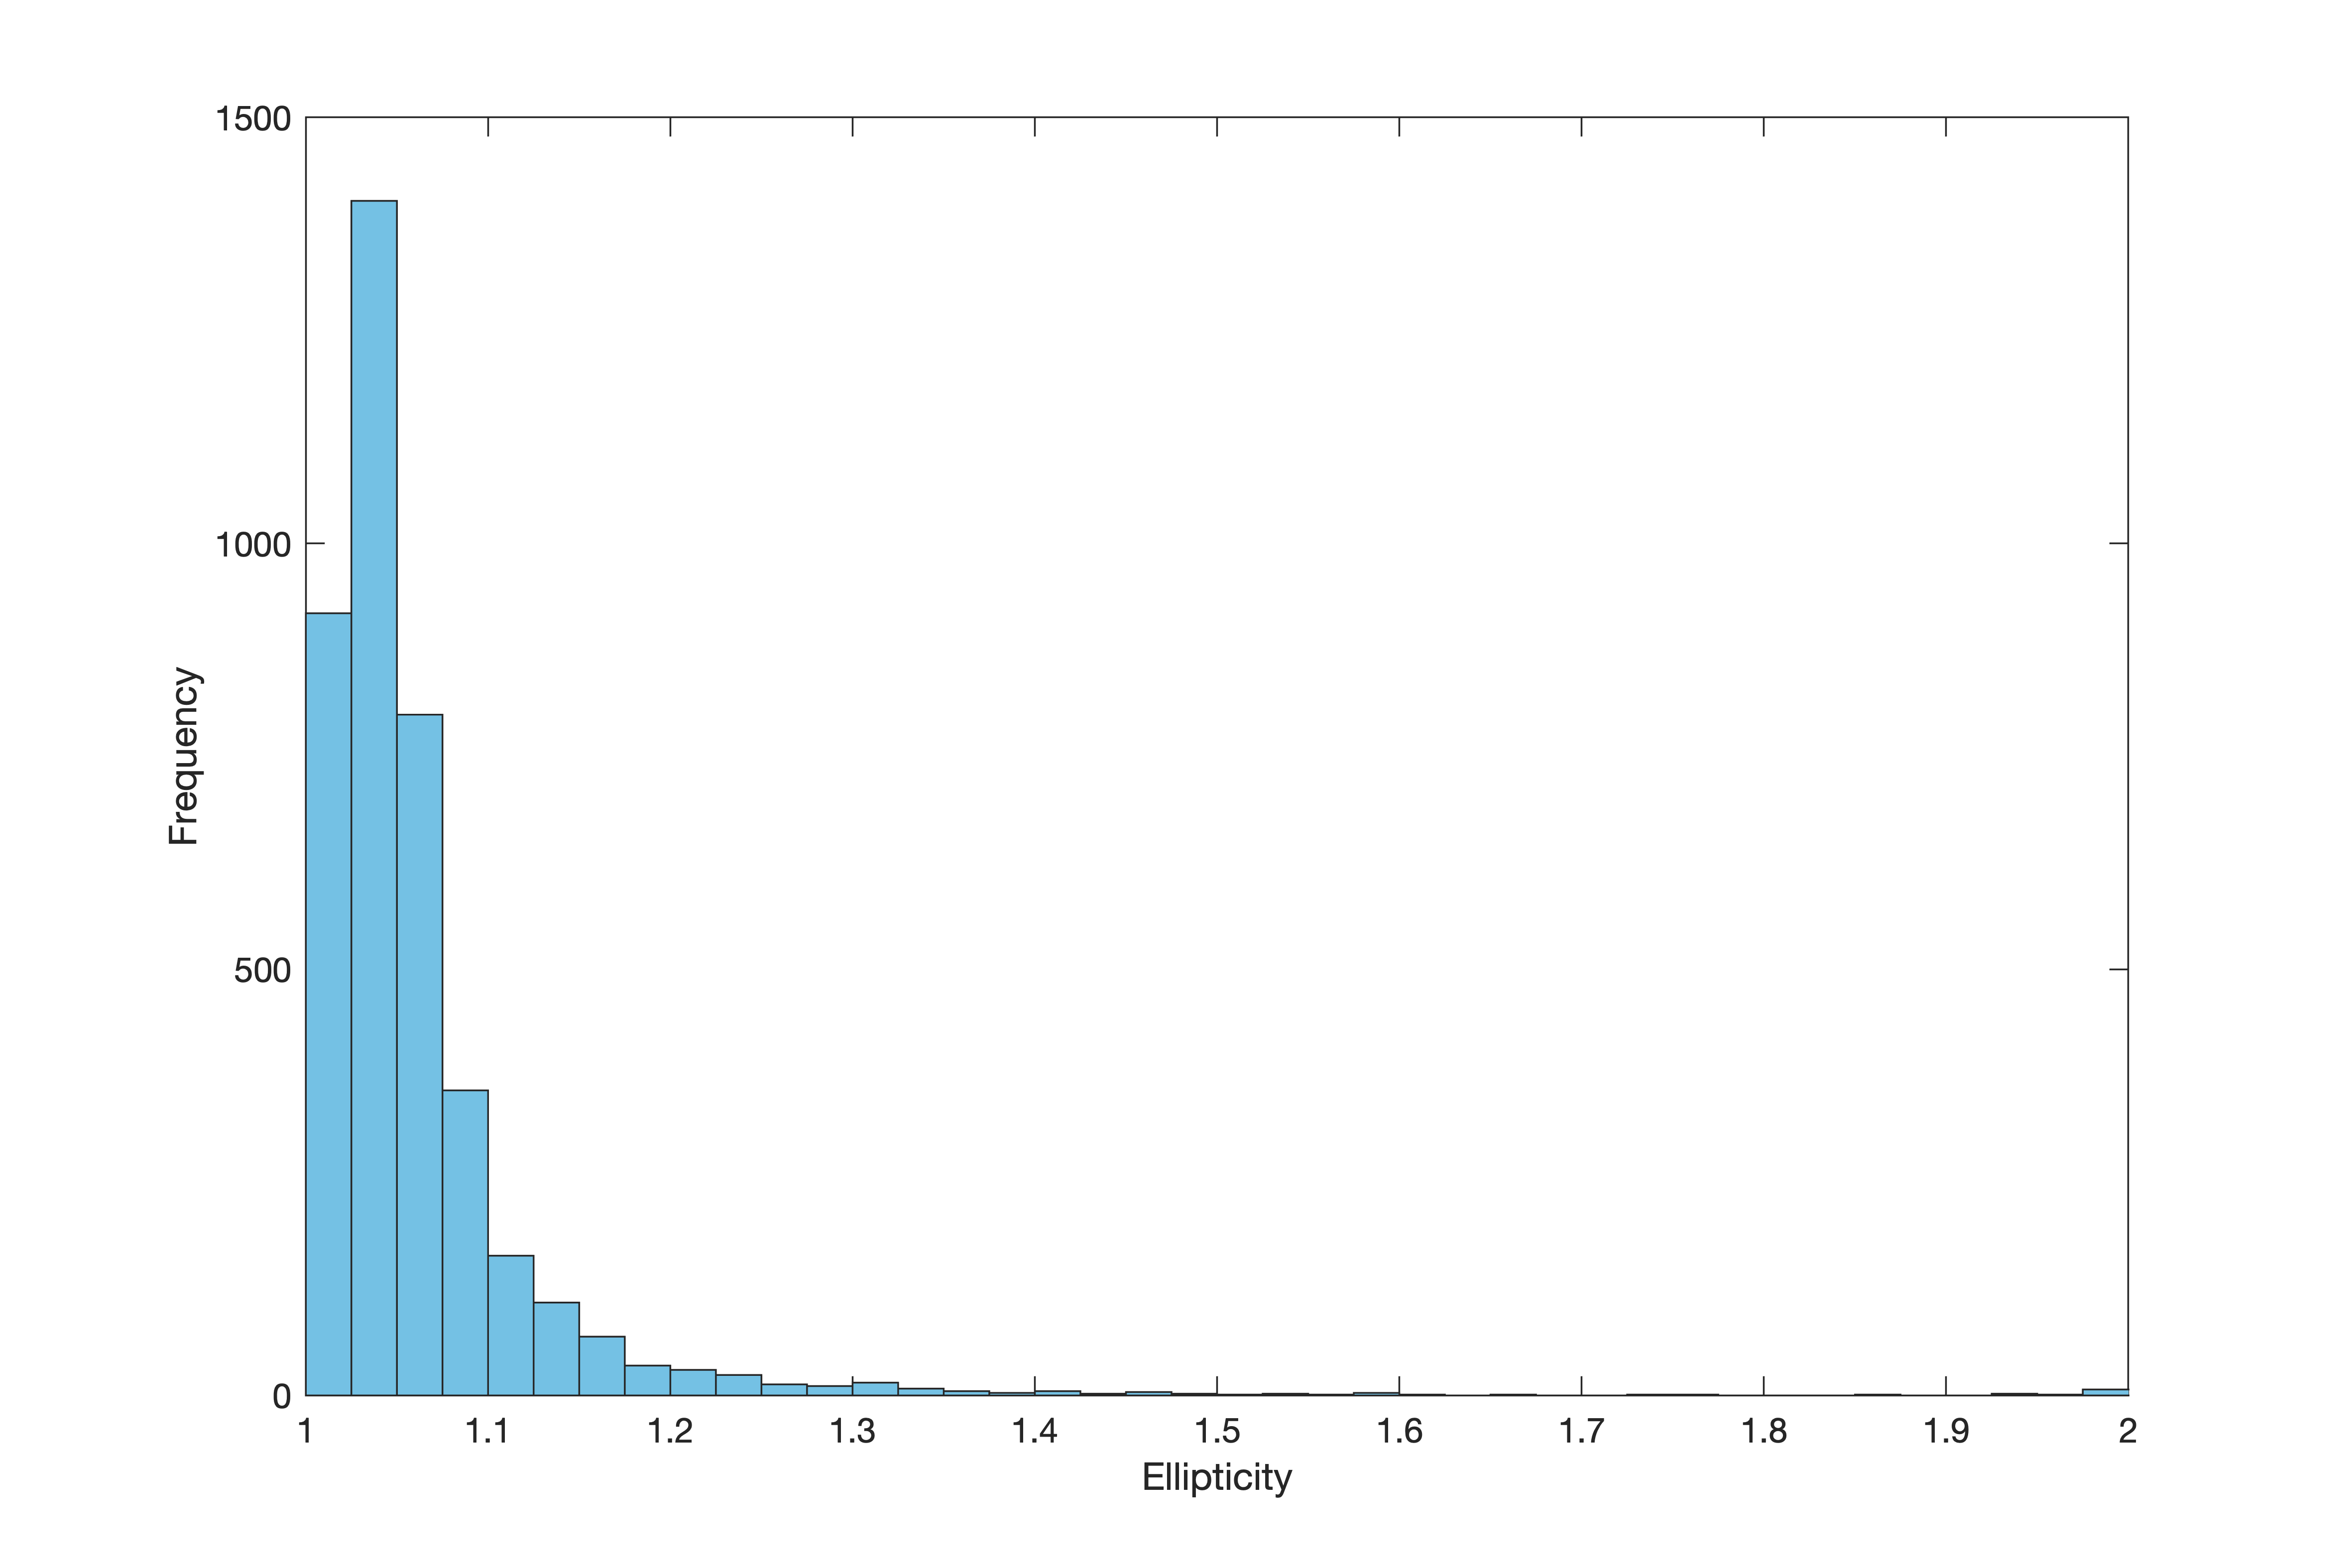
\includegraphics[width=\textwidth]{figures/fig2_4.png}
    \caption[Distribution of traced crater ellipticities]{Distribution of traced crater ellipticities.}
    \label{fig:2-4}
\end{figure}

\section{Adaptation of Holo et al. (2018)’s forward model}
\label{section:2-3}

To generate simulated crater azimuths, we adopted and modified \citet{holo2018a}’s forward cratering model. Their model consists of two parts: generating impactors and generating impacts under 91 different scenarios, each corresponding to holding Mars at a constant obliquity (each whole-number value in 0°--90°) over time. Because impact rates, impact angle distributions, and impact velocity distributions vary across the surface of Mars, Mars impacts exhibit latitudinal variations (such that cratering is more intensive at the poles than at the equator) \citep{lefeuvre2008a}. The oscillating obliquity of Mars adds a further layer of complication by shifting the positions of each latitude relative to the stream of impactors; this is how the various constant-obliquity simulations exerted an effect on the distribution of crater azimuths. The relationship between Mars obliquity, impactor direction of travel, and azimuth of resultant crater is visually diagrammed in Figure~\ref{fig:2-5}, based on Figure~1 in \citet{holo2018a}.

To generate impactors, \citet{holo2018a} assumed a steady state in the main asteroid populations, whose impacts they took to dominate the crater record on the surface of Mars \citep{bottke2000a, bottke2002a}. By running a Solar System simulation wherein modern Mars crossers were test particles and the planets were massive bodies, \citeauthor{holo2018a} retrieved 124 “close encounters,” defined as (the encounter speeds and encounter inclinations of) objects that passed within one Hill radius of Mars during the 10~Ma integration. From their 124 close encounters, we simulated $10^6$ impacts, then selected those resulting in elliptic crater formation ($\sim$80,000). These were then pared down to craters with diameters of at least 4~km ($\sim$20,000), whose latitude and azimuth were determined for 91 hypothetical constant-obliquity scenarios (each whole-number value in 0°--90°). The forward model therefore yielded an initial $91\times\sim20,000$ ensemble of elliptic crater azimuths, organized by constant-obliquity scenario. The impacting model is visually diagrammed in Figure~\ref{fig:2-6}, based on Figure~6 in \citep{holo2018a}.

Unlike \citet{holo2018a}, we subsequently tuned the initial output of the forward model such that the latitudinal distribution of the simulated craters better resembled that of collected crater data (§\ref{section:2-2}). While the 1,502 craters studied by \citet{holo2018a} spanned most of the latitudinal extent of Mars, this study’s measured (real) craters were located within specifically defined latitudinal boundaries. In the interest of having our simulated craters’ latitudinal distribution match that of our real craters, we devised a resampling procedure to normalize the simulated latitudinal distribution of craters to the empirical latitudinal distribution. The procedure entailed, first, sorting simulated craters into 5°-wide latitude bins and comparing the frequency of simulated craters within each latitude bin to the frequency of real craters within each latitude bin. (This procedure was applied for both the lAv and AHv units, which have different latitudinal distributions of craters, thereby resulting in two distinct sets of simulated craters.) Second, a scaling parameter was determined for each latitude bin as the empirical (i.e., desired) crater frequency divided by the simulated (i.e., pre-normalization) crater frequency. This scaling parameter was then divided by the maximum scaling parameter over all the latitude bins to yield a scaling factor $\le$1. Third, craters were resampled for each latitude bin; a random sample (without replacement) of the craters in each latitude bin was retained, and the rest discarded, where the proportion retained was the scale factor. Recall that there are two geologic units and 91 constant-obliquity scenarios; this procedure was therefore repeated for each geologic unit and each scenario separately. Finally, we scaled up the number of craters to $10^6$, by repeatedly randomly sampling (with replacement) the post-normalization set of craters, for each constant-obliquity scenario and each geologic unit, such that each final simulated crater ensemble had dimensions $91\times10^6$.

\begin{figure}
    \centering
    \includegraphics[width=\textwidth]{figures/fig2_5.png}
    \caption[Physical basis for variation in elliptic crater azimuth distribution]{Physical basis for variation in elliptic crater azimuth distribution by planetary obliquity scenario (north-south azimuths at low obliquity, left, and east-west azimuths at high obliquity, right). Meridian refers to any circle in the plane perpendicular to the equatorial plane. Based on Figure~1 in \citet{holo2018a}.}
    \label{fig:2-5}
\end{figure}

\begin{figure}
    \includegraphics[width=\textwidth]{figures/fig2_6.png}
    \caption[Schematic representation of the impact simulation model]{Schematic representation of the impact simulation model, wherein impactors are seeded in the disk and create craters on a location on Mars that varies with Mars obliquity. Because impactors are assumed to follow an orbit about the center of Mars that conserves angular momentum \citep{lefeuvre2008a}, all impactors within a disk with radius $\tau$, for a given $\{i_{\infty},v_{\infty}\}$, impact the surface. Note that the depicted impactor-seeding disk is only one of 124 such random disks, and impactors do not necessarily come at Mars from a specific angle to the orbital plane. Based on Figure~6 in \citet{holo2018a}.}
    \label{fig:2-6}
\end{figure}

\section{Determination of best-fit obliquity and geologic unit age}
\label{section:2-4}

Similar to Figure~7 in \citet{holo2018a}, we constructed crude probability density functions (i.e., histograms with bin width 10°) of the simulated crater azimuth distributions, one each for the lAv unit and the AHv unit. These represented the crater azimuth distributions we would expect to observe in our data given various hypothetical constant Mars obliquities. This alone would be insufficient to model Mars obliquity, however, because Mars obliquity has continuously oscillated.

To model the periodic (non-secular) oscillations of Mars obliquity, we therefore calculated the standard deviation of the past 2.5~Ma of Mars obliquity history, which we found to be 5.03° \citep{laskar2010a}. Applying this result, we resampled each constant-obliquity crater azimuth ensemble to fit a Gaussian distribution with its mean as the original obliquity and its standard deviation as 5.03°. Recall that the ensemble has dimensions $91\times10^6$; this resampling procedure was repeated for each $10^6$ set of craters such that the post-resampling set would consist of a mixture of craters from neighboring obliquities. For example, the resampled ensemble for 75° obliquity would consist of $10^6$ craters drawn, according to a Gaussian distribution centered around 75°, from a mixture of obliquity scenarios, such that $\sim$68~percent of the craters would come from obliquity scenarios between $\sim$70° and $\sim$80° and $\sim$95~percent of them would come from those between $\sim$65° and $\sim$85°. (Resampling also had the effect of significantly smoothing the subsequent $\chi^2$ tests that we performed.)

We applied the same procedure to construct histograms of the actual crater azimuth distributions, also finding the standard deviation, for each geologic unit. We then implemented 91 $\chi^2$ tests (one per obliquity scenario) for each geologic unit, comparing the simulated crater azimuth distributions to the real crater azimuth distributions. We took the obliquities for which the reduced $\chi^2$ statistic was at a minimum to be the best-fit mean obliquities, for each geologic unit. Using an curve intersection--finding script \citep{schwarz2017a}, we then found one--standard deviation confidence intervals graphically by determining the obliquities corresponding to a reduced $\chi^2$ statistic $\sqrt{2(8)}/8 = 0.5$ higher than the minimum (see §\ref{section:3-2}). Note that the variance of $\chi^2$ is defined as $2\nu$ where $\nu$ is the number of degrees of freedom (in this case, there were nine bins and one independent parameter, so $\nu=9-1=8$); the standard deviation of reduced $\chi^2$ is therefore 0.5.

The geologic units are described by \citet{tanaka2014a} as dating to the late Amazonian and Amazonian--Hesperian periods, respectively. To assign an absolute numeric age to each unit, however, we employed the isochron fitting criteria in Table~2 of \citet{michael2013a}, based on Martian epoch boundaries specified by \citet{hartmann2005a}. This entailed retrieving the density of craters with diameters larger than the relevant reference crater diameter (1~km) from \citet{tanaka2014a}, dividing that value by the relevant upper crater density boundary, and multiplying the fraction by the start of epoch specified by \citet{hartmann2005a}.

\section{Sensitivity checks}
\label{section:2-5}

As a primary sensitivity check, we reran the analyses to account for inter-analyst error in tracer azimuth tracing. The error in tracing was quantified by 23 repeat traces of craters by analyst 2 (Edwin Kite) in the AHv, using JMARS version 5.2, of which five were found to be elliptic based on the 1.05 threshold. In addition, we searched the 1,502 elliptic craters from Appendix C in \citet{holo2018a}, sourced from the \citet{robbins2012a} database, finding four which analyst 1 had traced in the procedure outlined in §\ref{section:2-2}. We thus computed the nine differences between the azimuth values of analyst 1's original traces with analyst 2’s and with those used by \citet{holo2018a}. We then applied at random an inter-analyst perturbation (one of the nine differences, or their negative counterpart, such that there were 18 options for perturbation) to each crater azimuth (see §\ref{section:4-3}). In practice, this meant iterating through analyst 1--traced crater azimuths and randomly adding or subtracting one of the nine inter-analyst differences to create a new set of crater azimuths. The perturbed dataset was then passed through the same procedure outlined in §\ref{section:2-4} for comparison with simulations. As an additional sensitivity check, we also reran the analyses, filtering traced craters using various threshold ellipticities (the default 1.05, as well as the higher thresholds of 1.10 and 1.15, in addition to the no-threshold case, 1.00, included for interest).

\chapter{Results}
\label{chapter:3}

\section{Simulated and observed crater azimuth distributions}
\label{section:3-1}

Figure~\ref{fig:3-1} shows the simulated and actual crater azimuth distributions, represented by line plot histograms, for the lAv unit and AHv units. For clarity, only select obliquity scenarios are shown. Both the original crater data and the inter-analyst-perturbed data are shown.

\begin{figure}
    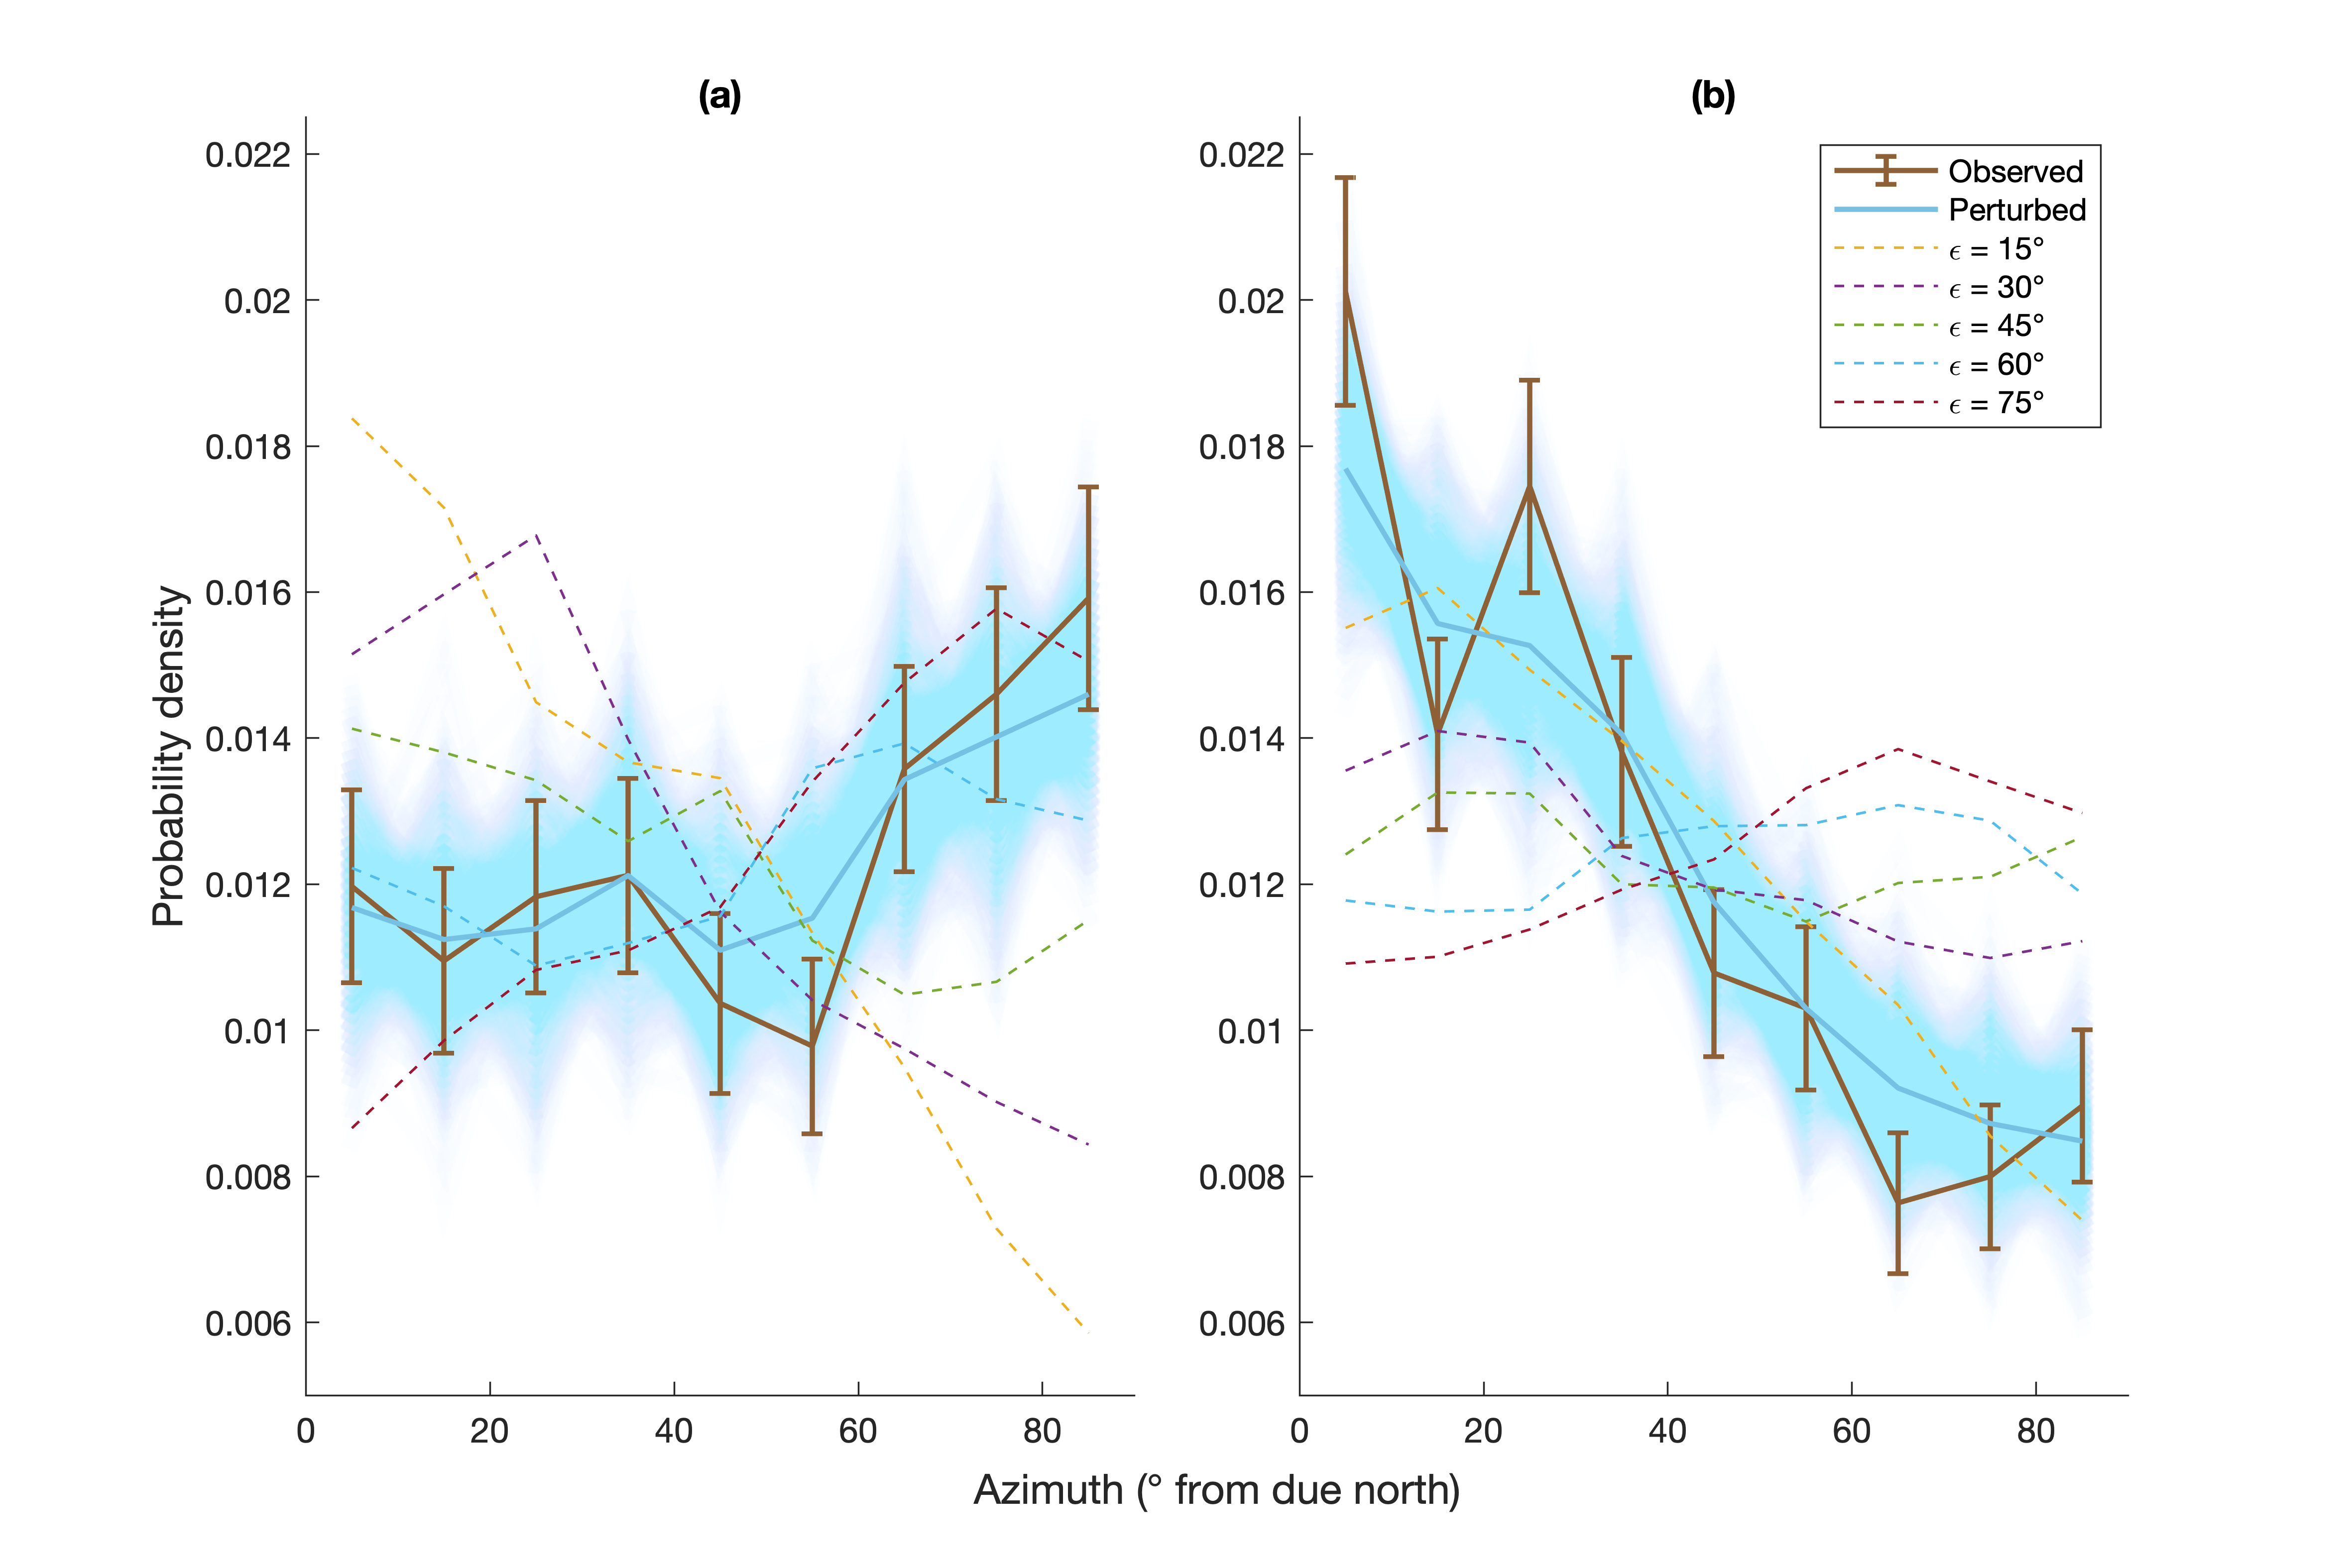
\includegraphics[width=\textwidth]{figures/fig3_1.png}
    \caption[Distribution of simulated and observed crater azimuths]{Distribution of simulated and observed crater azimuths for the (a) lAv and (b) AHv units. Dotted lines: simulated, Gaussian-resampled, latitude distribution--normalized obliquity scenarios for different mean obliquities, $\epsilon$; translucent turquoise lines: 1,000 random instances of inter-analyst-perturbed observed crater azimuths; solid blue line: median of the 1,000 perturbed azimuths.}
    \label{fig:3-1}
\end{figure}

\section{Simulated--observed crater azimuth distribution comparisons}
\label{section:3-2}

Figure~\ref{fig:3-2} shows the extent of mismatch (the reduced $\chi^2$ statistic) of each Gaussian-smoothed obliquity scenario, for each geologic unit, where a lower mismatch $\sim 1$ indicates a better simulation--data fit. Both the results from the original crater data and those from the inter-analyst-perturbed data are shown. The results of the $\chi^2$ tests are summarized in Table~\ref{tab:3-1}.

\begin{figure}
    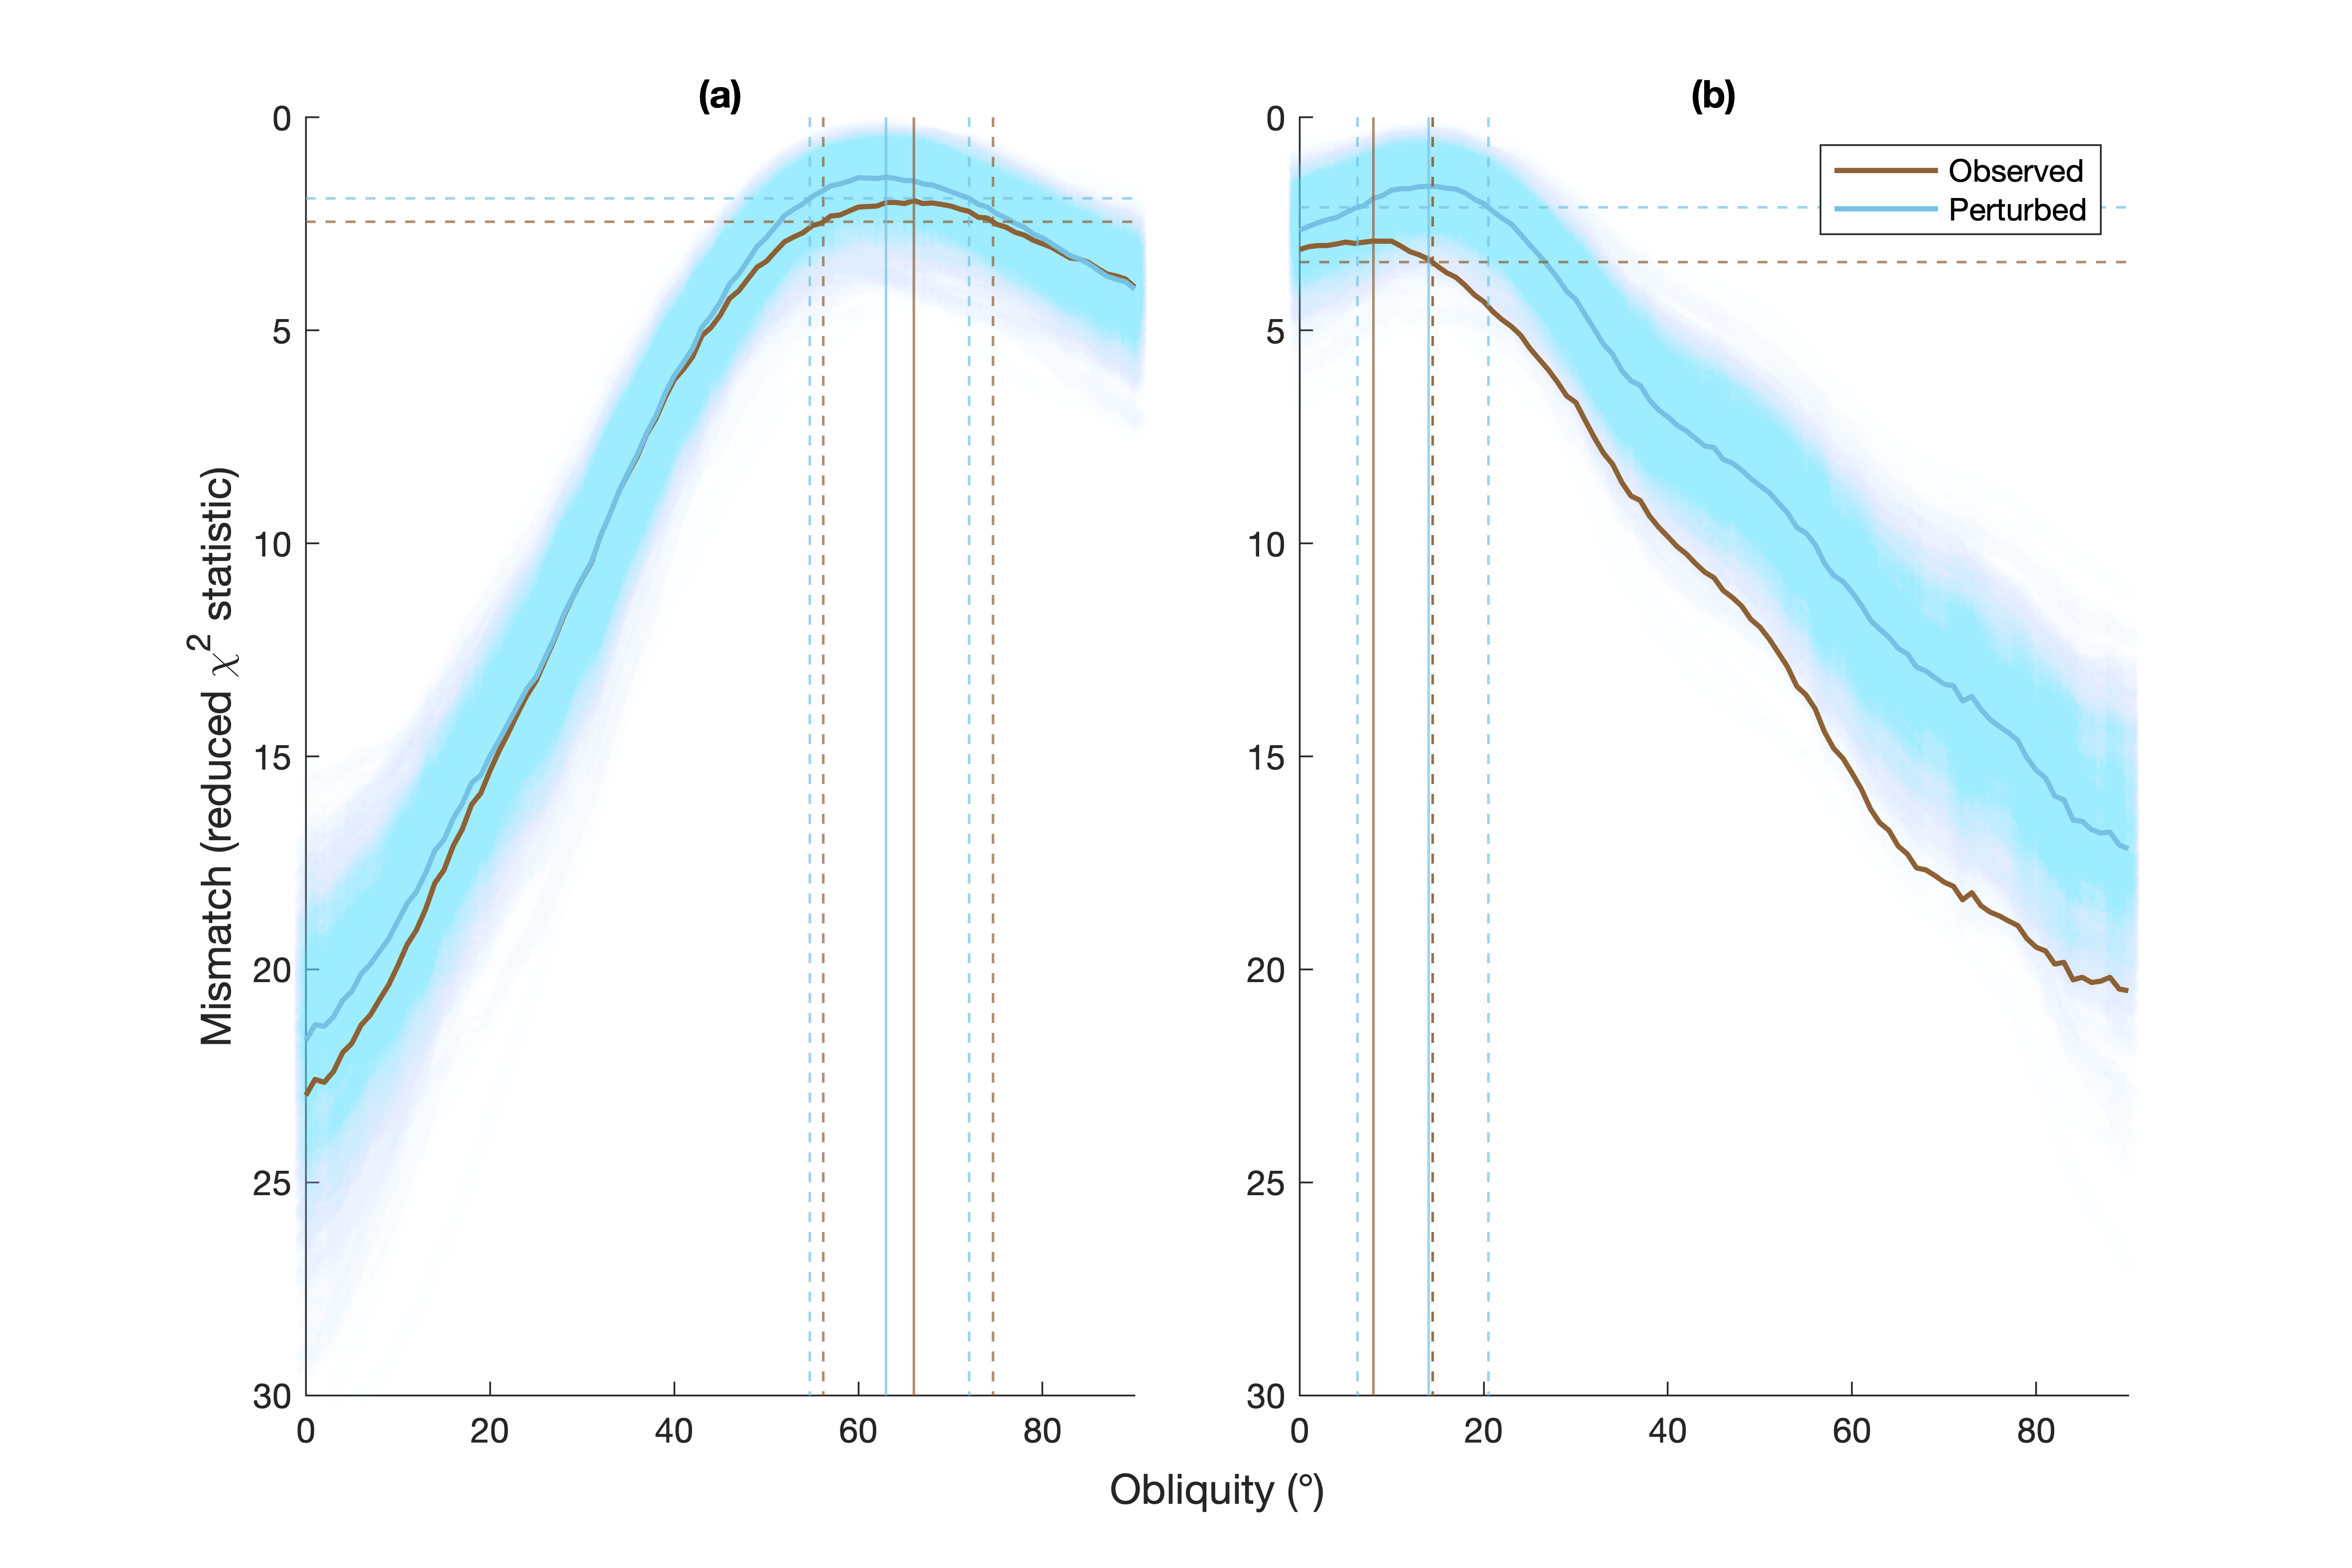
\includegraphics[width=\textwidth]{figures/fig3_2.png}
    \caption[Mismatch between the simulated and observed crater azimuth distributions]{Mismatch (reduced $\chi^2$ statistic) between the crater azimuth distribution of each Gaussian-smoothed obliquity scenario and the observed crater azimuth distribution for the (a) lAv and (b) AHv units. Translucent turquoise lines: 1,000 random instances of inter-analyst-perturbed observed crater azimuths; solid blue line: median of the 1,000 perturbed azimuths; central, solid vertical lines: best-fit obliquity, corresponding to the minimum reduced $\chi^2$ statistic; the dotted vertical lines: confidence interval.}
    \label{fig:3-2}
\end{figure}

\begin{table}
    \centering
    \caption[Summary of simulated--observed mismatch results for crater azimuth distribution]{Summary of results of $\chi^2$ tests between simulated crater azimuth distributions and the observed crater azimuth distribution.}
    \label{tab:3-1}
    \bigskip
    \begin{tabular}{
        c
        c
        S[table-format=2.1]
        S[table-format=2.0]
        S[table-format=2.1]
    }
    \toprule
    \thead{Geologic unit} & \thead{Description} & \multicolumn{1}{c}{\thead{Lower\\ bound (°)}} & \multicolumn{1}{c}{\thead{Best fit\\ (°)}} & \multicolumn{1}{c}{\thead{Upper\\ bound (°)}} \\
    \midrule
    \multirow{2}{*}{lAv} & Original trace & 56.2 & 66 & 74.6 \\
                         & Inter-analyst-perturbed & 54.7 & 63 & 72.0 \\
    \multirow{2}{*}{AHv} & Original trace & 0.0 & 8 & 14.4 \\
                         & Inter-analyst-perturbed & 6.3 & 14 & 20.5 \\
 \bottomrule
    \end{tabular}
\end{table}

\section{Mean obliquity of Mars over geologic time}
\label{section:3-3}

Table~\ref{tab:3-2} summarizes the absolute unit ages of each geologic unit. Figure~\ref{fig:3-3} summarizes the mean obliquity over time corresponding to each geologic unit, based on simulation--data comparisons from §\ref{section:3-2}, also plotting the deterministic reverse integrations provided by \citet{laskar2010a}.

\begin{figure}
    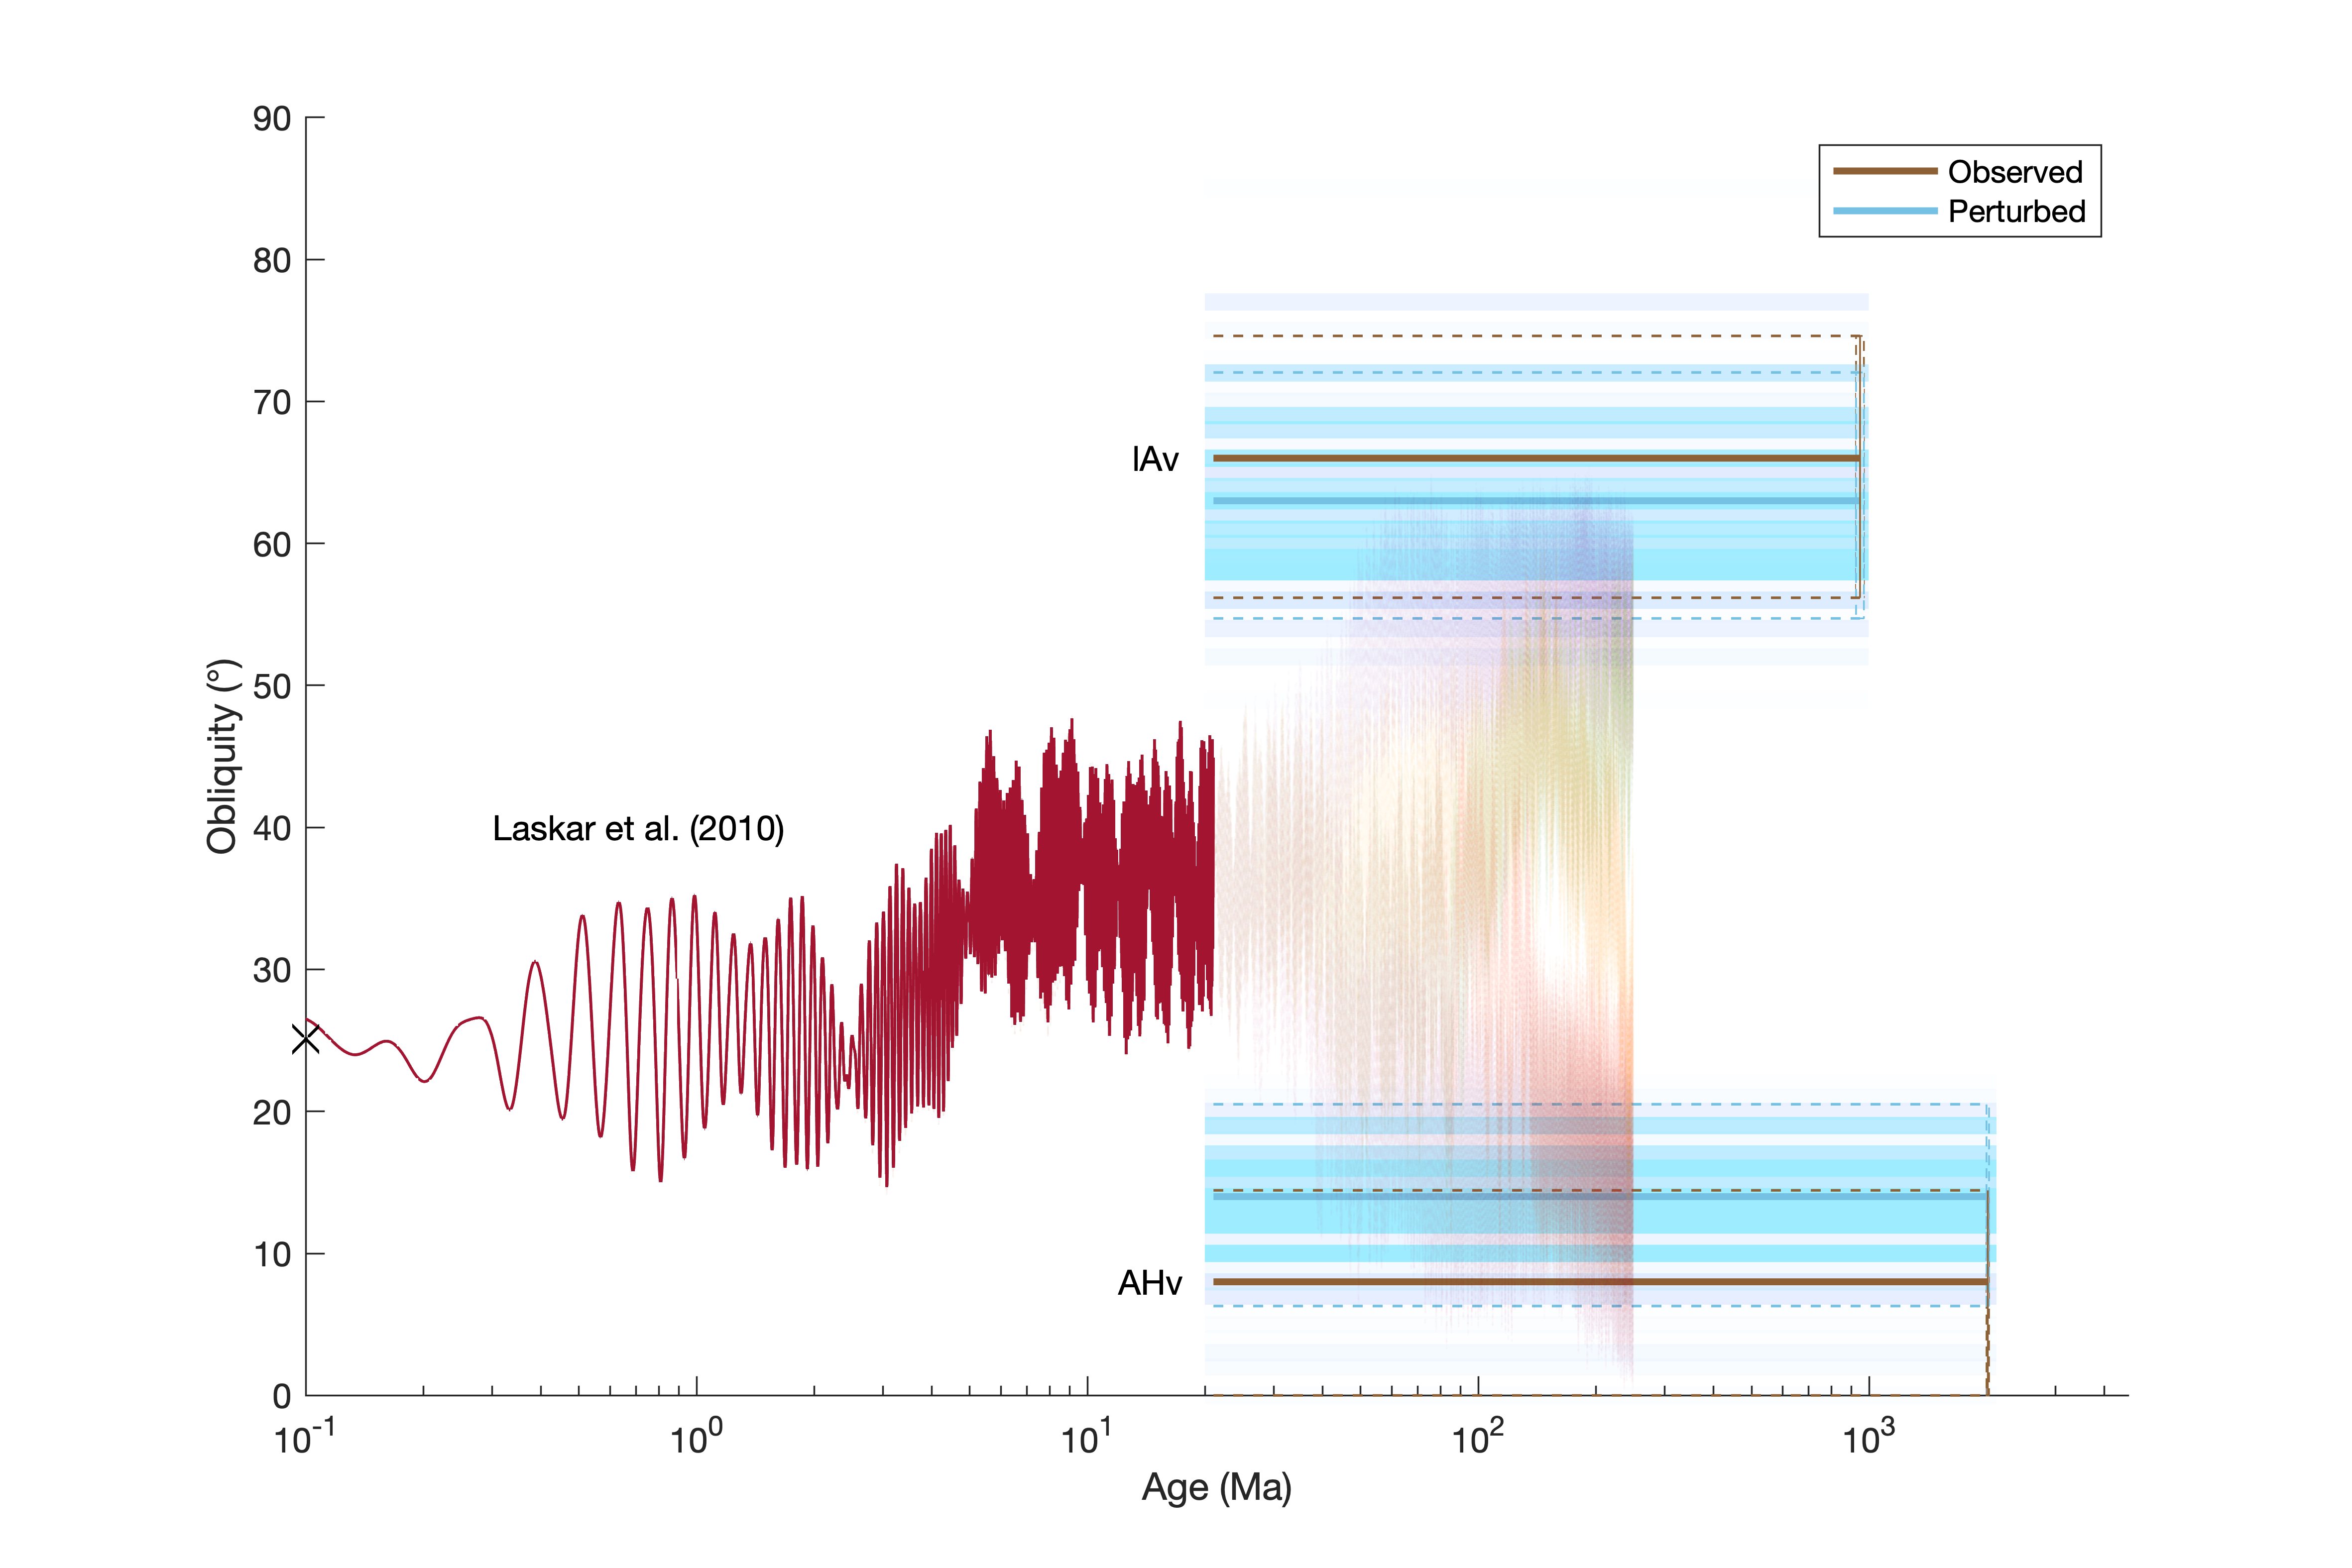
\includegraphics[width=\textwidth]{figures/fig3_3.png}
    \caption[Mean obliquity of Mars over time (logarithmic scale)]{Mean obliquity of Mars over time (logarithmic scale). Translucent turquoise: estimates based on 1,000 random instances of inter-analyst-perturbed observed crater azimuths; blue: best-fit mean obliquity for the median of the 1,000 perturbed azimuths (solid line: best fit; dotted lines: upper and lower confidence bounds with respect to standard deviation); brown: best-fit mean obliquity estimates for the original crater traces (solid line: best fit; dotted lines: upper and lower bounds with respect to standard deviation); black cross: present-day obliquity (25.1°); burgundy: \citet{laskar2010a}’s deterministic reverse integration; other translucent lines: five chaotically diffusive reverse integrations to 249~Ma ago, demonstrating that large swings in Mars obliquity, due to secular spin-orbit resonances, make it impossible to precisely reverse-integrate its history beyond $\sim$100~Ma.}
    \label{fig:3-3}
\end{figure}

\begin{table}
    \centering
    \caption{Absolute ages of sampled geologic units.}
    \label{tab:3-2}
    \bigskip
    \begin{tabular}{
        c
        S[table-format=4.1, table-alignment=right]@{\ \ \( \pm \)}
        S[table-format=3.1, table-alignment=left]
        S[table-format=1.3]@{\,\( \pm \)\,}
        S[table-format=1.3]
    }
    \toprule
        \thead{Geologic\\ unit} & \multicolumn{2}{c}{\thead{Density of craters\\ with diameter >1~km,\\ $N(1)$ (per Mkm\textsuperscript{2})}} & \multicolumn{2}{c}{\thead{Absolute age\\ (Ga)}} \\
    \midrule
        lAv & 551.8 & 12.7 & 0.947 & 0.022 \\
        AHv & 1303.3 & 9.9 & 2.011 & 0.015 \\
    \bottomrule
    \end{tabular}
\end{table}

\chapter{Discussion}
\label{chapter:4}

\section{Synthesis of results}
\label{section:4-1}

Simulations of Mars crater azimuths exhibit a pattern whereby the crater population is more north-south oriented at lower obliquities and more east-west oriented at higher obliquities (Figures~\ref{fig:2-5}, \ref{fig:3-1}). This pattern (of sensitivity of azimuth distribution to obliquity) holds much more strongly for the lAv unit than for the AHv unit. In other words, for the lAv unit, histograms show that more extreme obliquities are associated with more lopsided (heavily north-south or east-west oriented) azimuth distributions; by contrast, for the AHv unit, histograms for obliquities 30°, 45°, 60°, and 75° all show roughly flat azimuth distributions. The simulations for the two geologic units only differ because crater samples were sourced from different latitudes: craters in the lAv unit spans latitudes $\sim$0--45° (north and south were folded), while traced craters in the AHv unit comprise separate low-latitude ($\sim$0°--25°) and high-latitude ($\sim$40--65°) subsets (Figure~\ref{fig:4-1}); it thus appears that higher-latitude crater azimuths are less sensitive to obliquity.

As shown in Figure~\ref{fig:3-3}, Mars’s recent (past $\sim$100~Ma) obliquity trajectory lies between an early historical (past $\sim$2.0~Ga) low period, followed by a later historical (past $\sim$0.9~Ga) high period. In particular, Figure~\ref{fig:3-2} indicates statistically that Mars’s mean obliquity recorded on the lAv unit (i.e., since $\sim$0.9~Ga ago) has likely been very high, at $\sim$66° (56.2°--74.6° standard deviation interval), and that recorded on the AHv unit (i.e., since $\sim$2.0~Ga ago) very low, at $\sim$8° (0.0°--14.4° standard deviation interval). For the AHv specifically (Figure~\ref{fig:3-2}b), there is also an especially notable offset between the mismatches of the inter-analyst-perturbed and those of non-perturbed crater azimuth data, possibly due to the more extreme azimuths, and consequently more extreme mean obliquity, determined from the non-perturbed crater data (see §\ref{section:4-3}). For each geologic unit, the smallest $\chi^2$ value, implying the least mismatch, is not sharply defined. Indeed, although standard deviation confidence intervals are defined more precisely, very low $\chi^2$ values (<5) are observed through the high obliquity range of $\sim$40° and up for the lAv unit, and likewise through the low obliquity range of $\sim$25° and under for the AHv unit. This study is consequently unable to rule out large swaths of possible past mean obliquities, although the result that the older unit is associated with lower obliquity than the younger unit is clear. 

\begin{figure}
    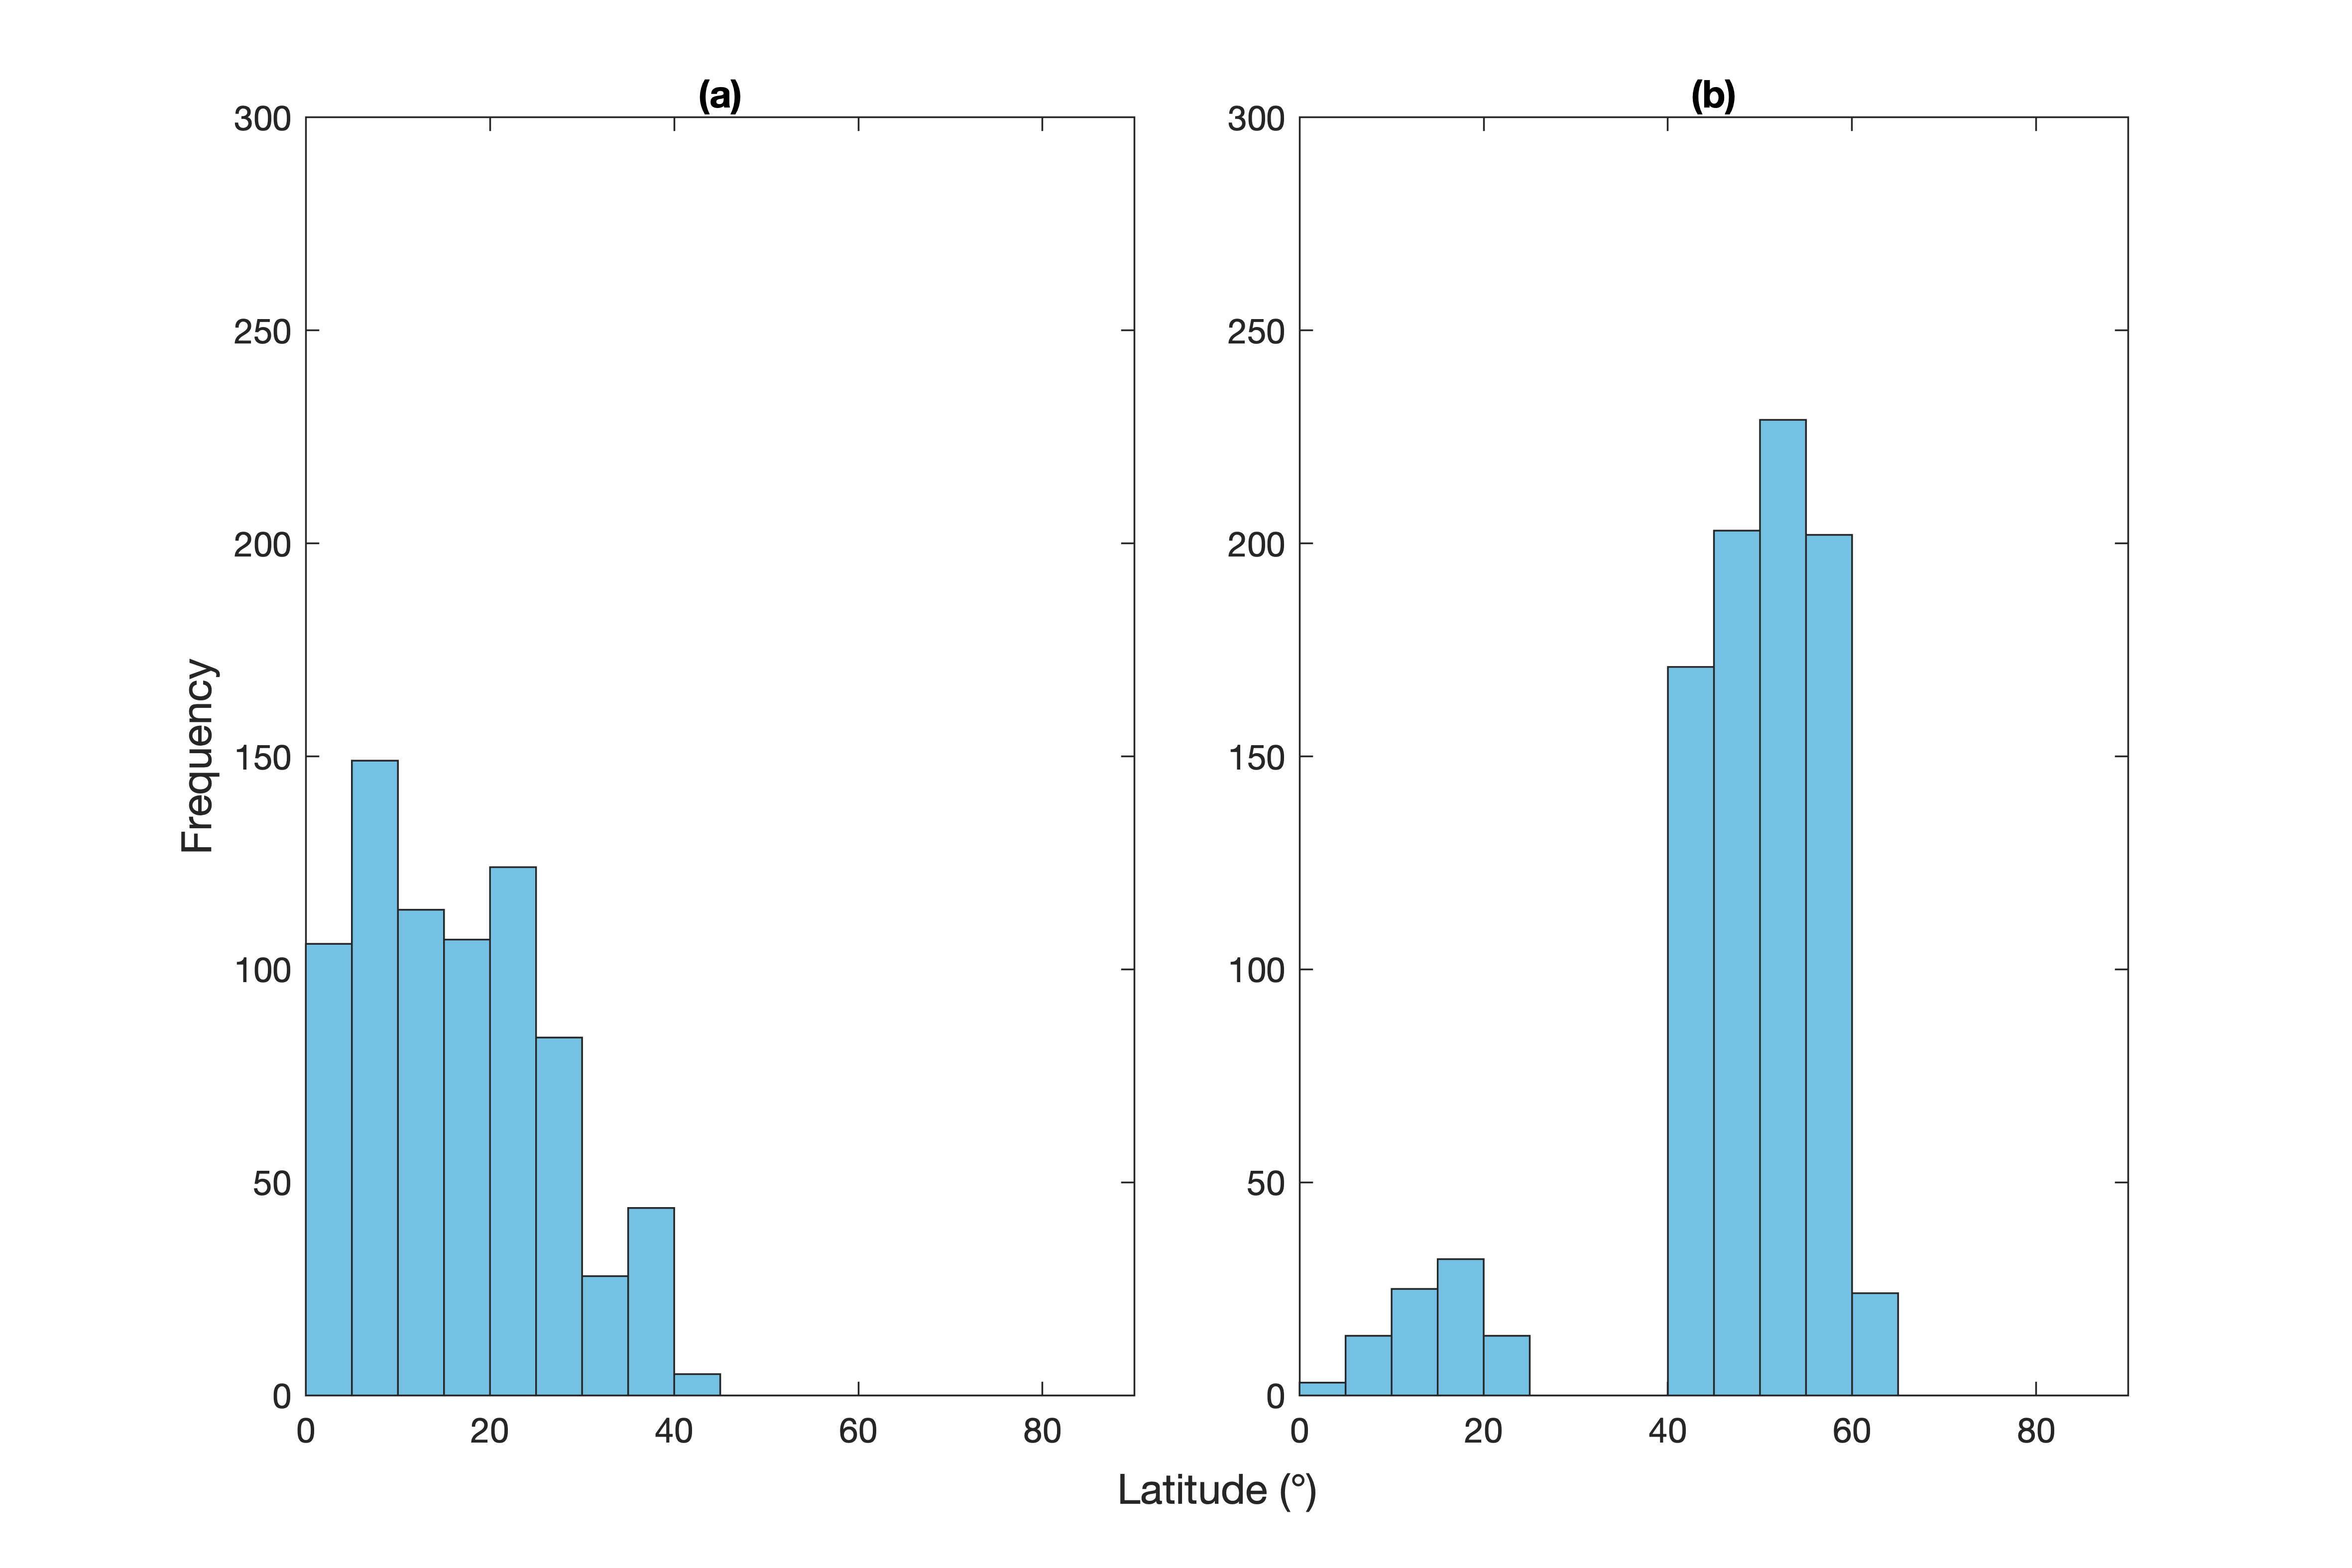
\includegraphics[width=\textwidth]{figures/fig4_1.png}
    \caption[Latitude frequency histogram of traced craters]{Frequency histogram showing the number of elliptic craters traced per 5° latitude bin for the (a) lAv and (b) AHv units.}
    \label{fig:4-1}
\end{figure}

\section{Comparison with previous studies}
\label{section:4-2}

\citet{holo2018a} estimated that the mean obliquity over the past $\sim$3.5~Ga was likely between $\sim$10° and $\sim$30°. The confidence interval of our best-fit mean obliquity approximation for the older AHv unit, 0.0° to 14.4°, aged $\sim$2.0~Ga, is consistent with, albeit firmly at the lower end, of the previous estimate. It is possible that a higher-obliquity excursion from $\sim$3.5~Ga ago to $\sim$2.0~Ga ago could have pulled the mean obliquity to a higher value for the entire post--late Hesperian period, which could be investigated using older geologic units. However, \citeauthor{holo2018a} also estimated that the fraction of time spent at obliquities >40° was less than one-fifth of the time since $\sim$3.5~Ga ago. This is most likely inconsistent with our 56.2° to 74.6° mean obliquity estimate for Mars since $\sim$0.9~Ga ago, which represents well over one-fifth of the time elapsed since $\sim$3.5~Ga ago.

While our impacting forward model was based on that of \citet{holo2018a}, we employ different methods for comparing forward-model simulated crater data and real crater data. \citeauthor{holo2018a} assigned weightings to different obliquity histories based on how many times each history provides the best fit (using the two-sample Kolmogorov--Smirnov test) to a bootstrapped sample of the real crater data, then take the weighted averages of those obliquity histories to find the mean obliquity since $\sim$3.5~Ga ago. By contrast, this study instead makes direct comparisons between the simulated crater azimuth distributions, for each whole-number value of obliquity in 0°--90°, and the real crater azimuth distributions. Further research should therefore cross-examine these studies’ methodologies by applying the method of \citet{holo2018a} to our data, and vice versa, to investigate the extent to which methodological differences explain the likely inconsistencies in outcome.

\citet{laskar2010a} additionally provided five solutions to 249~Ma ago in order to demonstrate the chaotic diffusion of Mars obliquity at >100~Ma timescales. Of these, two solutions exhibited relatively low mean obliquities ($\sim$27° and $\sim$20°), while three solutions exhibited relatively high mean obliquities ($\sim$39°, $\sim$51°, and $\sim$41°); however, none had a periodic mean obliquity >60° (Figure~\ref{fig:3-2}a). While these chaotic backward integrations do not give any indication of the validity of our results, they demonstrate that high-obliquity excursions are a feasible outcome of chaotic obliquity variation, thus indicating that a 56.2° to 74.6° mean obliquity since $\sim$0.9~Ga cannot be \textit{a priori} ruled out.

\section{Sensitivity tests}
\label{section:4-3}

First, we performed inter-analyst sensitivity tests showing that our results were robust to random perturbation, even though the inter-analyst comparison of elliptic crater azimuths revealed significant discrepancies (Figures~\ref{fig:3-1}, \ref{fig:3-2}, \ref{fig:3-3}; Table~\ref{tab:3-1}). As Table~\ref{tab:4-1} shows, three of the nine elliptic craters retraced by analyst 2 or also available in Appendix C of \citet{holo2018a} yielded a greater-than-15° azimuth difference when compared with analyst 1's original traces. However, it is unlikely that these resulted from systematic biases, because non--analyst 1 azimuths are not uniformly larger or smaller than analyst 1 azimuths. Differences in traced elliptic crater azimuths could have arisen from eroded or unclear crater rims, as well as from quirks in \citet{gal2003a}’s ellipse-fitting script.

The inter-analyst-perturbed results were generally more moderate (i.e., indicating obliquities further from the extremes of 0° and 90°) than the results based on the original traces. This was due to the symmetric nature of azimuths; for example, given an absolute inter-analyst difference of 20°, perturbing an azimuth of 85° by $+$20° would result in a new azimuth of 75°, while perturbing it by $-$20° would result in a new azimuth of 65°; either way, the new azimuth would be further from the extremes of 0° to 90°. In addition, the inter-analyst-perturbed results generally exhibit better fits with the simulated azimuth distributions, with smaller $\chi^2$ values uniformly for all obliquities and both geologic units (Figure~\ref{fig:3-2}).

Further consideration of the implications of §\ref{section:4-1}---that over the past $\sim$2.0~Ga the mean obliquity was just 8°, but that over that past $\sim$0.9~Ga it was 66°---in fact necessitates the inclusion of the inter-analyst-perturbed results in the overall results for the study’s conclusions to be feasible: since obliquities range from 0° to 90°, the $\sim$1.06~Ga period extending from $\sim$2.0~Ga ago to $\sim$0.9~Ga ago would have to have had a negative mean obliquity, which is unphysical. This inconsistency possibly reflects methodological problems, including the imprecise tracing and unrepresentative selection of craters (such that the observed azimuths were too extreme); the incorrect dating of geologic units (for instance, dating the lAv unit to be substantially younger than $\sim$0.9~Ga, e.g., $\sim$0.20~Ga, would result in a positive mean obliquity during the intervening $\sim$1.81~Ga period from $\sim$2.0~Ga ago to $\sim$0.20~Ga ago); and possible issues with the forward model (see §\ref{section:4-5}).

Second, as discussed in §\ref{section:2-2}, we tested the effect of varying the ellipticity threshold (1.05 in our main procedure) on our results. Filtering for craters with ellipticity >1.10 (yielding 521 craters) and >1.15 (yielding 248), we found decreasingly similar crater azimuth distributions for each geologic unit (Figure \ref{fig:4-2}). Note that, because only two of the nine craters whose inter-analyst variability was quantified had ellipticity >1.10, we were not able to perform inter-analyst sensitivity checks on the 1.10- and 1.15-threshold results. With a 1.10 ellipticity threshold, we found mean obliquities associated with the AHv, at 1° (0.0° to 17.6 standard deviation interval), and with the lAv, at 53° (42.0° to 75.3° standard deviation interval), to be lower than our 1.05-threshold results; while with a 1.15 threshold, we found mean obliquities of 0° (0.0° to 30.0° standard deviation interval) and 45° (25.9° to 65.0° standard deviation interval), respectively (Table \ref{tab:4-2}). These tests indicate a negative relationship of ellipticity threshold with mean obliquity associated with the lAv and no clear relationship with mean obliquity associated with the AHv; however, it is likely that sample sizes become too small to draw conclusions from at thresholds beyond 1.05, as shown by the increasing flatness of the reduced $\chi^2$ statistic distributions (Figure \ref{fig:4-3}). For interest, results for the no-threshold case are also given.

\begin{table}
    \centering
    \caption{Inter-analyst variability in traced elliptic crater azimuths.}
    \label{tab:4-1}
    \bigskip
    \begin{tabular}{
        @{}
        c
        S[table-format=2.1]
        S[table-format=2.1]
        S[table-format=2.1]
        S[table-format=2.1]
        S[table-format=2.1]
        S[table-format=2.1]
        S[table-format=2.1]
        S[table-format=2.1]
        S[table-format=2.1]
        @{}
    }
    \toprule
        \thead{Crater No.} & \multicolumn{1}{c}{\thead{1}} & \multicolumn{1}{c}{\thead{2}} & \multicolumn{1}{c}{\thead{3}} & \multicolumn{1}{c}{\thead{4}} & \multicolumn{1}{c}{\thead{5}} & \multicolumn{1}{c}{\thead{6}} & \multicolumn{1}{c}{\thead{7}} & \multicolumn{1}{c}{\thead{8}} & \multicolumn{1}{c}{\thead{9}} \\
    \midrule
        Analyst 1 (°) & 54.7 & 56.9 & 29.0 & 60.1 & 22.1 & 23.6 & 63.2 & 28.0 & 21.2 \\
        Analyst 2 (°) & 22.7 & 61.2 & 22.5 & 50.7 & 40.4 & & & & \\
        \citet{holo2018a} (°) & & & & & & 49 & 62 & 31 & 19 \\
        Absolute difference (°) & 32.0 & 4.4 & 6.5 & 9.4 & 18.3 & 25.4 & 1.2 & 3.0 & 2.2 \\
    \bottomrule
    \end{tabular}
\end{table}

\begin{figure}
    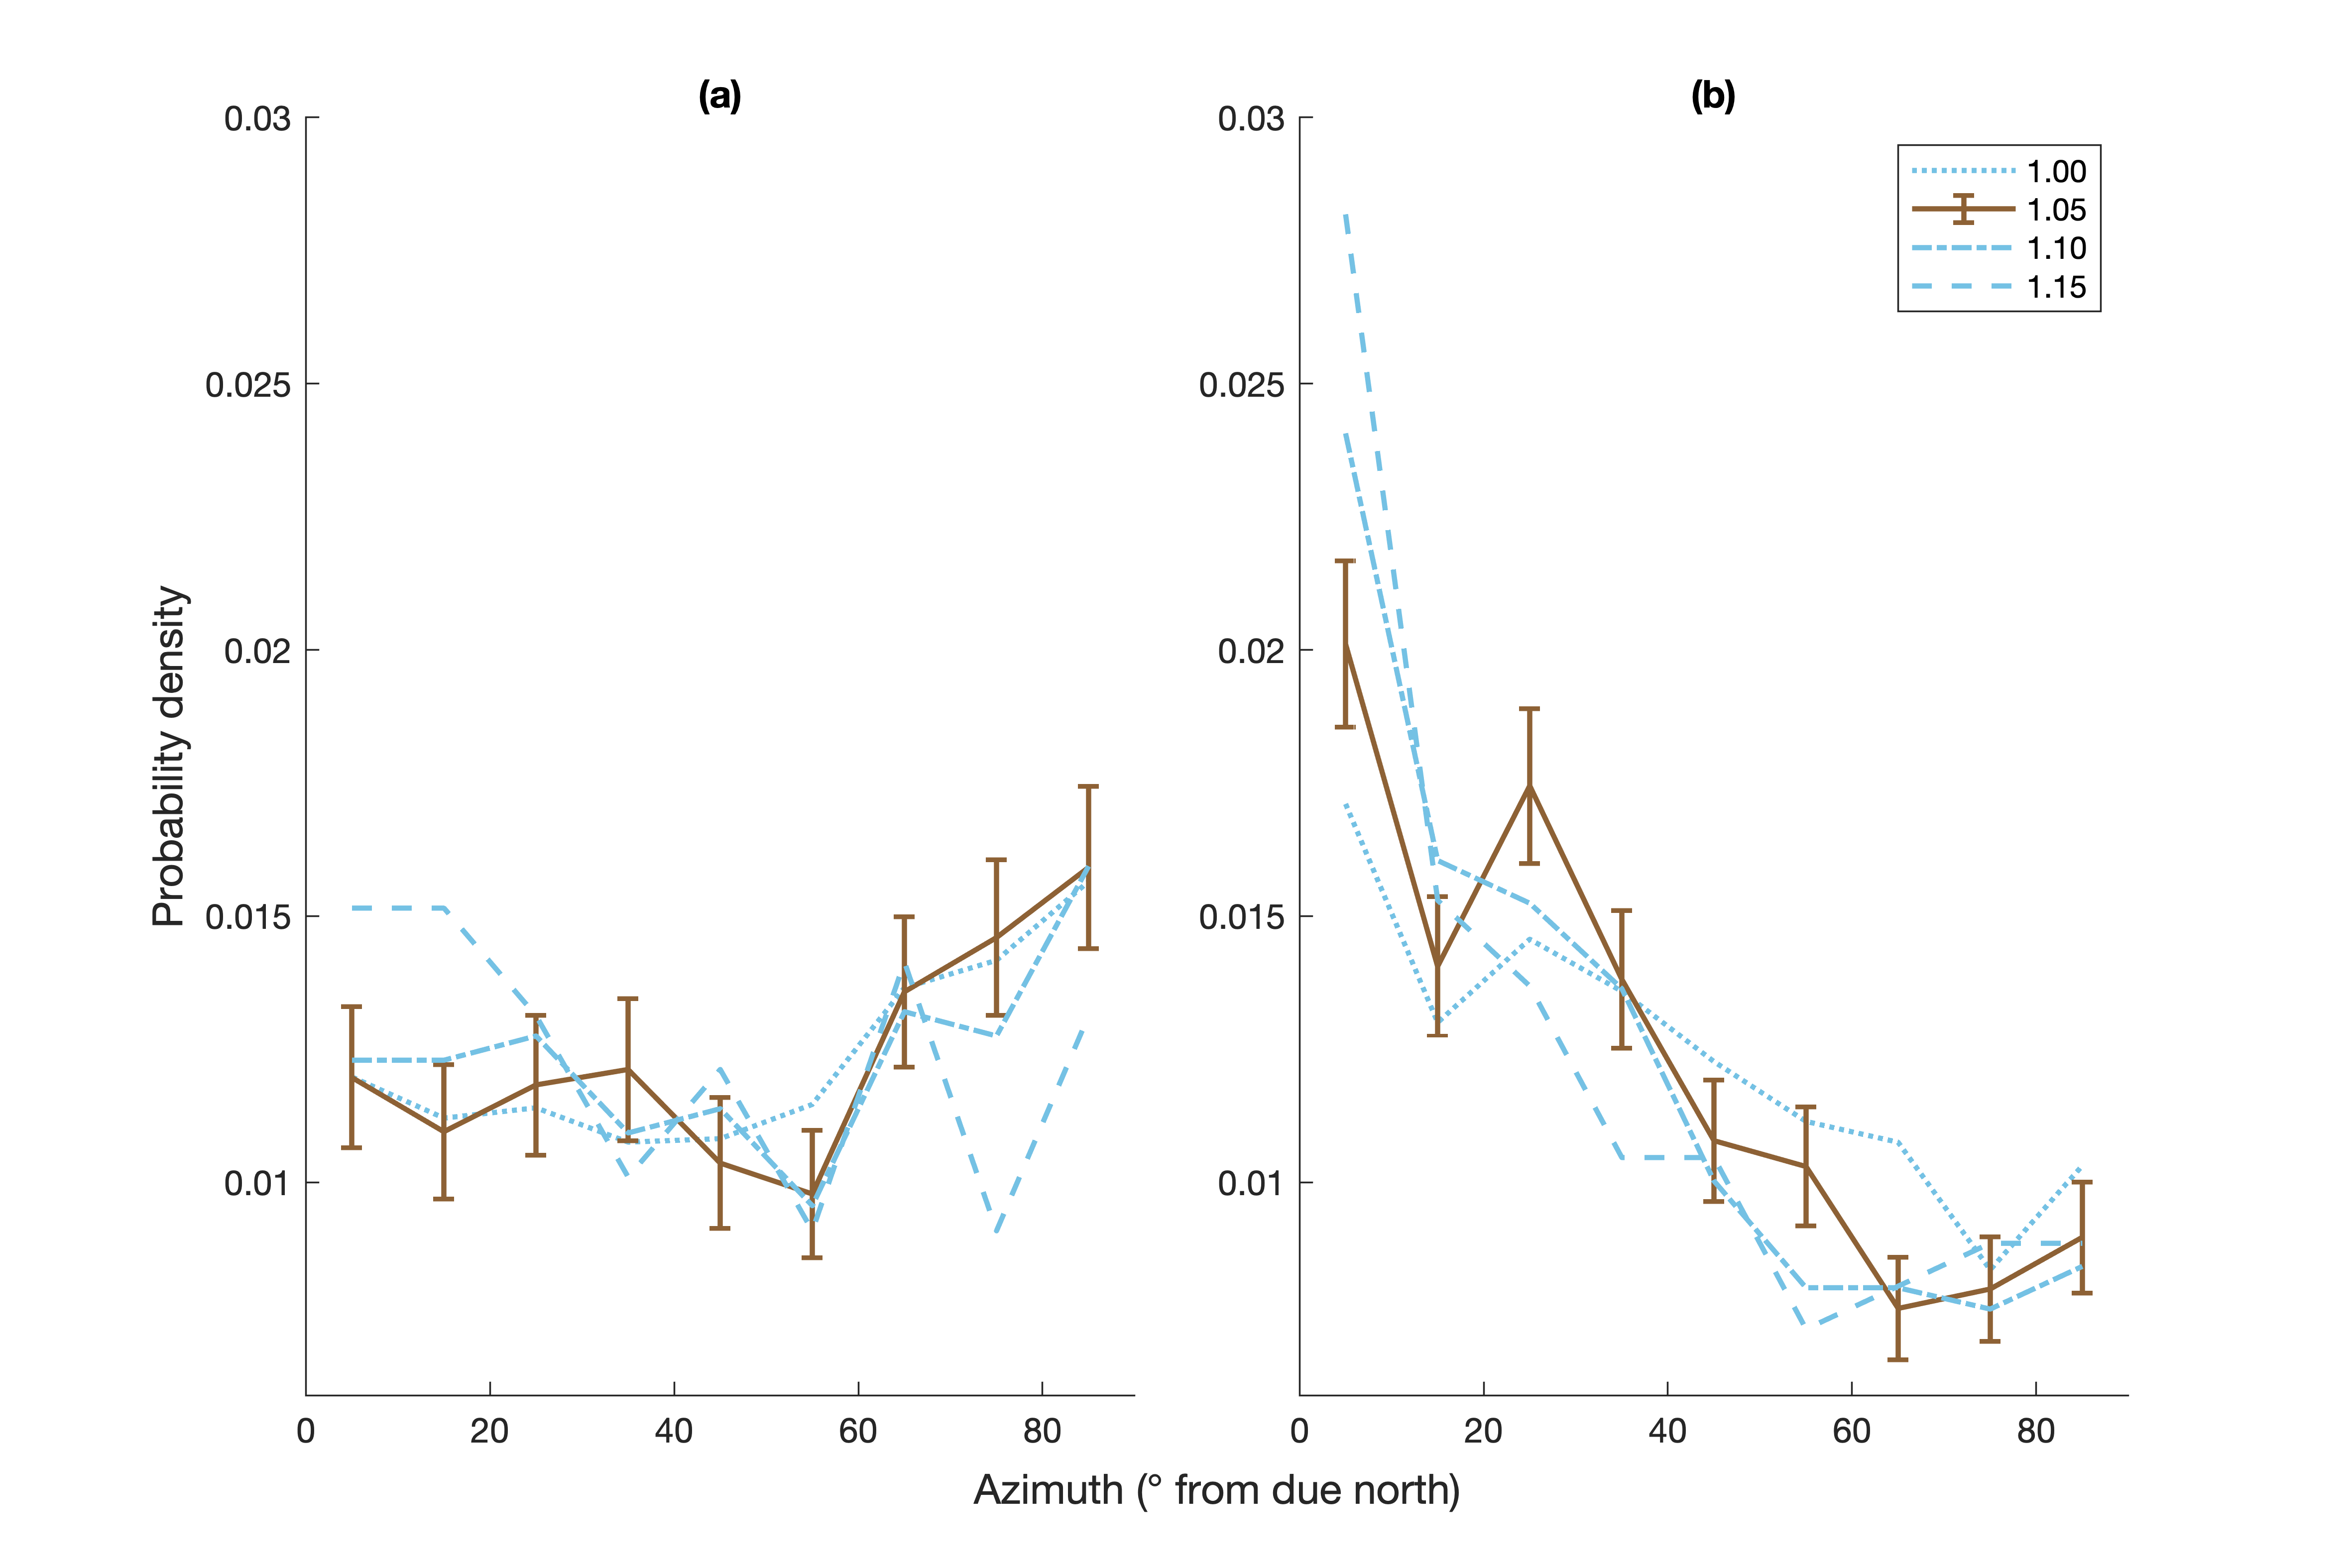
\includegraphics[width=\textwidth]{figures/fig4_2.png}
    \caption[Distribution of observed crater azimuths by ellipticity threshold]{Distribution of observed crater azimuths for various ellipticity thresholds, for the (a) lAv and (b) AHv units.}
    \label{fig:4-2}
\end{figure}

\begin{table}
    \centering
    \caption[Simulated--observed crater azimuth distribution mismatch by threshold ellipticity]{Summary of results of $\chi^2$ tests between simulated crater azimuth distributions and the observed crater azimuth distribution for various threshold ellipticities.}
    \label{tab:4-2}
    \bigskip
    \begin{tabular}{
        c
        c
        S[table-format=4.0]
        S[table-format=2.1]
        S[table-format=2.0]
        S[table-format=2.1]
    }
    \toprule
    \thead{Threshold ellipticity} & \thead{Geologic unit} & \multicolumn{1}{c}{\thead{Crater count}} & \multicolumn{1}{c}{\thead{Lower\\ bound (°)}} & \multicolumn{1}{c}{\thead{Best fit\\ (°)}} & \multicolumn{1}{c}{\thead{Upper\\ bound (°)}} \\
    \midrule
    \multirow{2}{*}{1.00} & lAv & 1726 & 59.2 & 65 & 69.7 \\
                          & AHv & 2273 & 19.1 & 22 & 26.4 \\
    \multirow{2}{*}{1.05} & lAv & 761 & 56.2 & 66 & 74.6 \\
                          & AHv & 917 & 0.0 & 8 & 14.4 \\
    \multirow{2}{*}{1.10} & lAv & 244 & 42.0 & 53 & 75.3 \\
                          & AHv & 277 & 0.0 & 4 & 11.9 \\
    \multirow{2}{*}{1.15} & lAv & 110 & 25.9 & 45 & 65.0 \\
                          & AHv & 138 & 0.0 & 0 & 30.0 \\
    \bottomrule
    \end{tabular}
\end{table}

\begin{figure}
    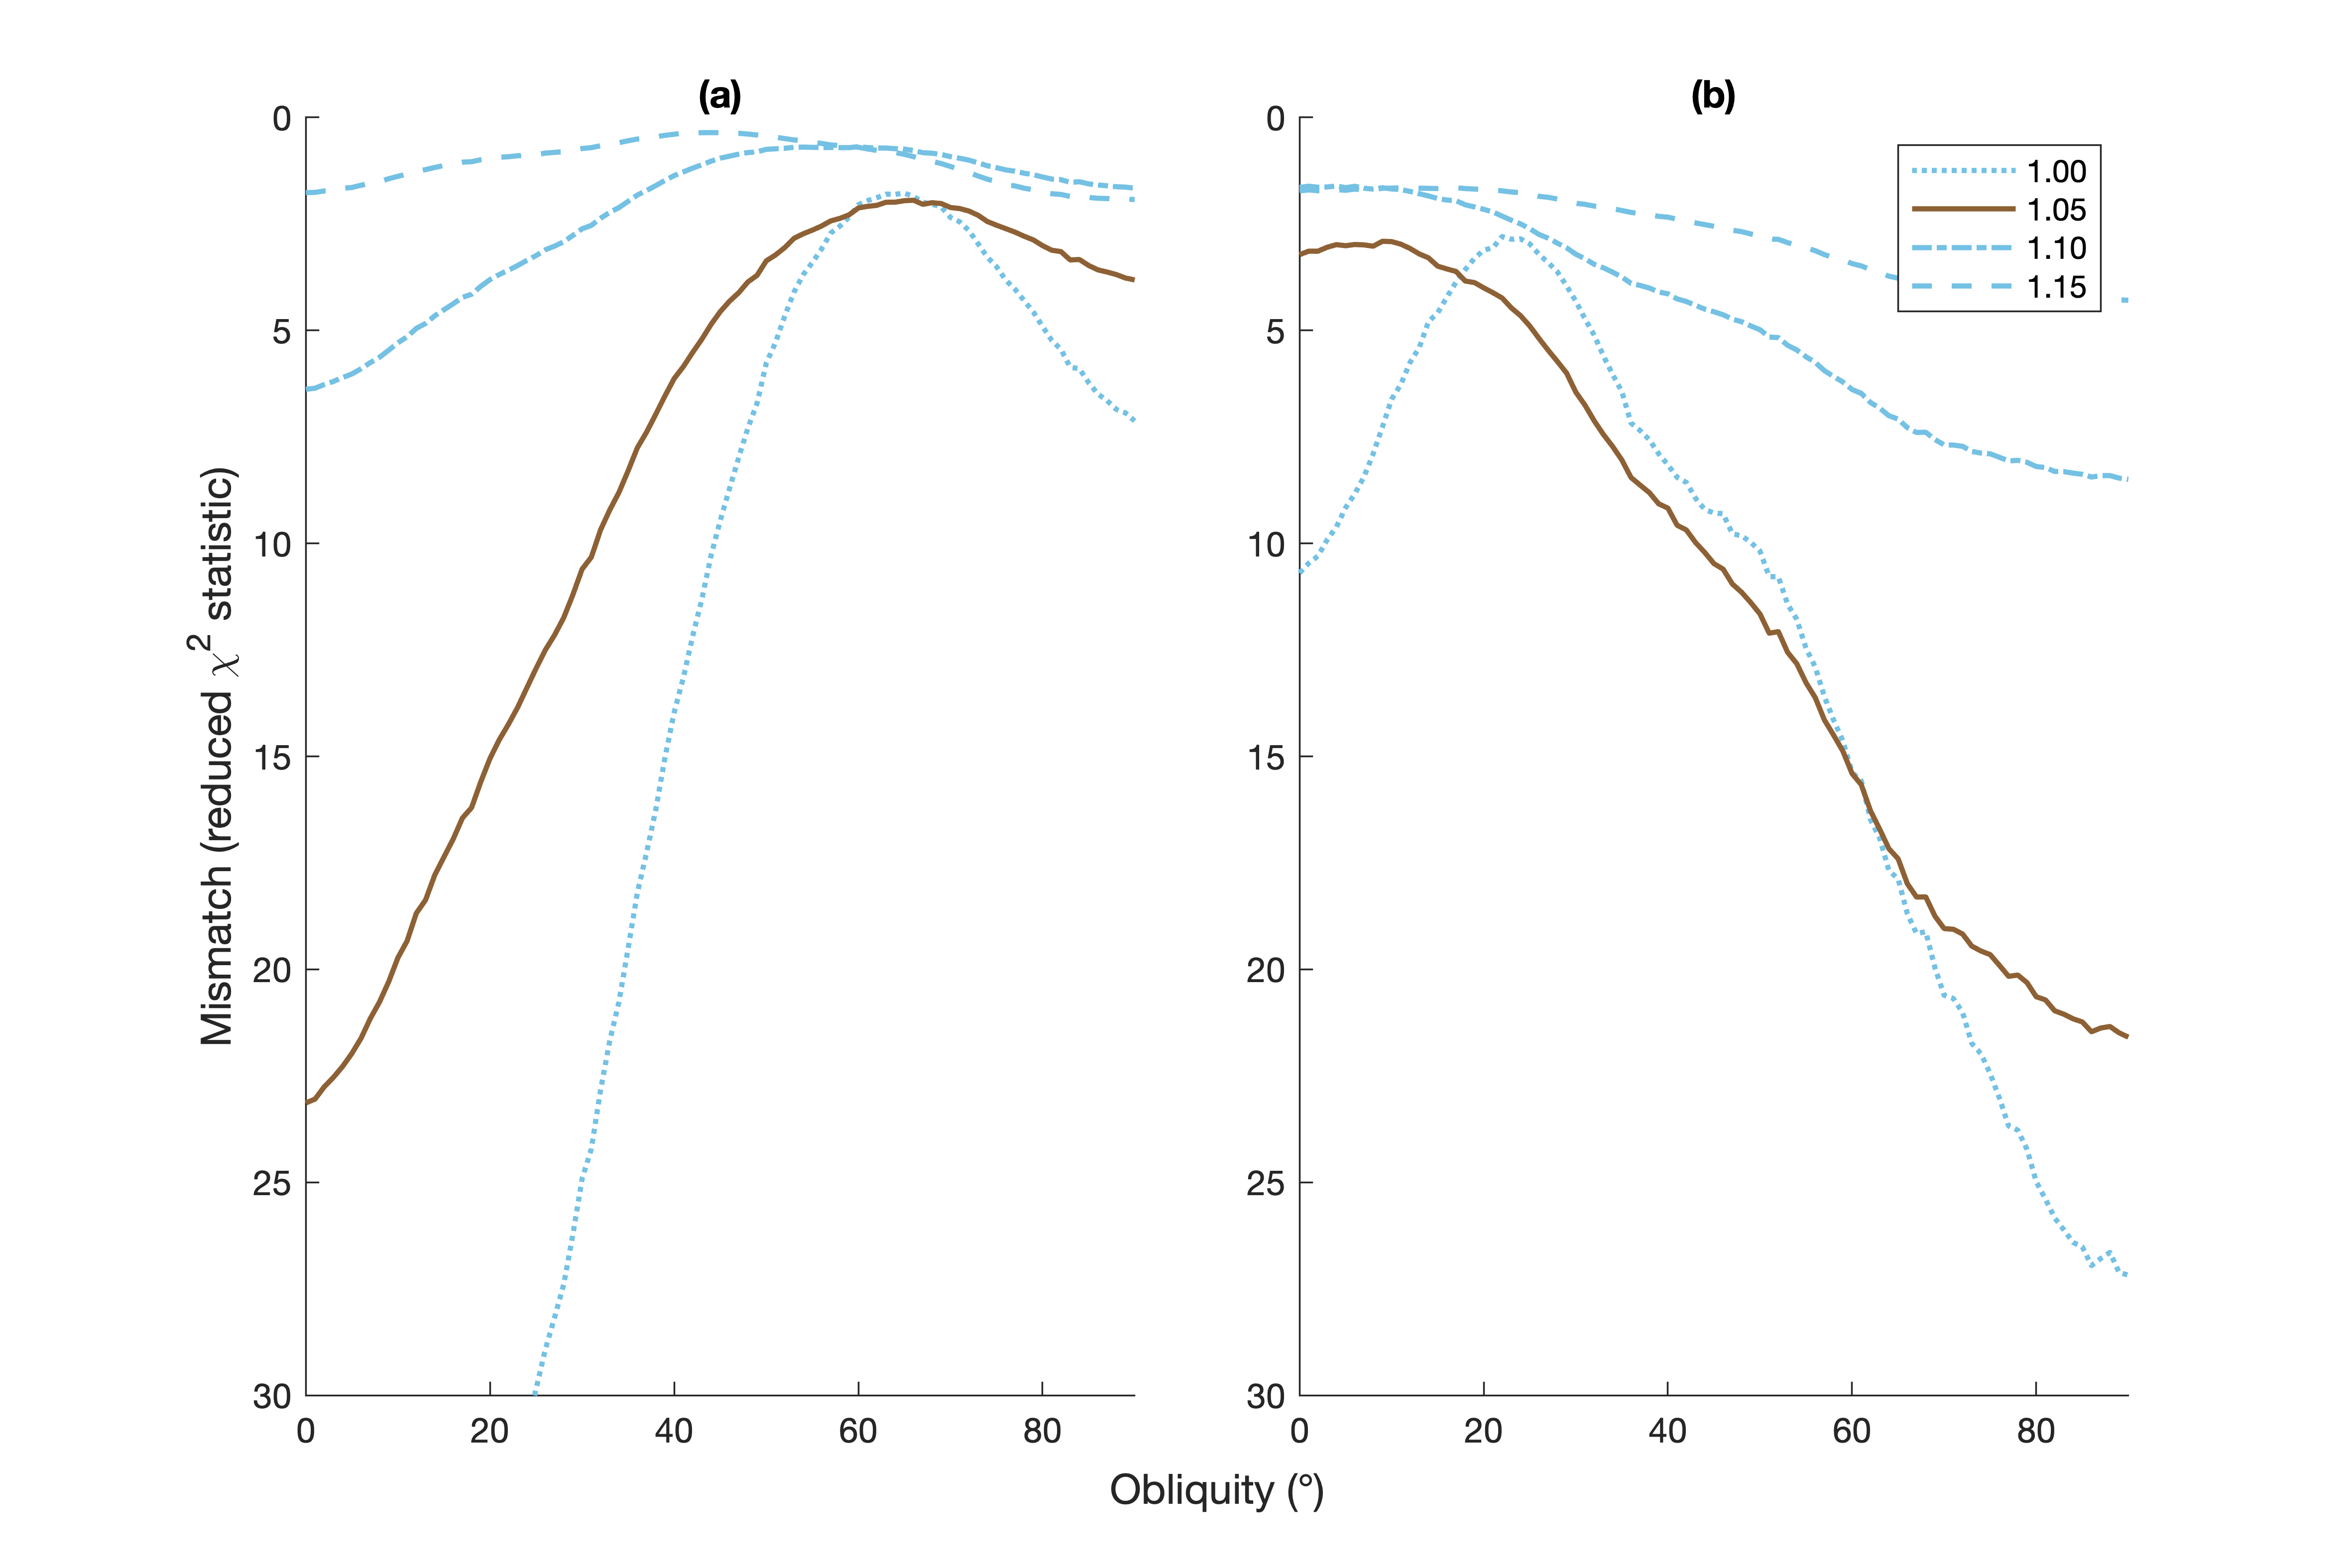
\includegraphics[width=\textwidth]{figures/fig4_3.png}
    \caption[Simulated--observed crater azimuth distribution mismatch by ellipticity threshold]{Simulated--observed crater azimuth distribution mismatch (reduced $\chi^2$ statistic) for various ellipticity thresholds, for the (a) lAv and (b) AHv units.}
    \label{fig:4-3}
\end{figure}

\section{Implications of results}
\label{section:4-4}

As reviewed in §\ref{section:1-3}, the implications for surface volatiles on Mars of high and low obliquity excursions are well understood (reviewed in Jakosky, 2021) and are caused by changes in insolation patterns by latitude: the higher latitudes receive more, and the lower latitudes receive less, insolation at higher obliquity, and vice versa. Our results indicate that Mars has experienced extensive high and low obliquity periods in its distant geologic past, such that a number of scenarios are possible. For instance, during its earlier low-obliquity period associated with the AHv unit, when its poles would have been better shielded from the Sun, Mars may have been more likely to harbor extensive glacial ice sheets at its poles, thus thinning out the atmosphere by precipitating gaseous CO2 and causing atmospheric collapse at the poles, while also experiencing greater desiccation of deep aquifers \citep{lindner1985a, kreslavsky2005a, phillips2011a, soto2015a, grimm2017a}; while, during its later high-obliquity period associated with the lAv unit, Mars may have seen greater sublimation of water ice, the migration of water ice to its lower latitudes, and a higher water vapor pressure, in addition to more frequent polar dust storms \citep{haberle1990a, jakosky1995a, zent2013a, forget2017a}.

\citet{fassett2014a}, studying craters superposed on glacial deposits, triangulated the timing of the extensive deposition of ice in the mid-latitudes to the middle to late Amazonian. Because this latitudinal pattern of ice deposition is associated with relatively high obliquities, their result suggests that the mean middle to late Amazonian obliquity was relatively high. Our result is consistent with \citet{fassett2014a} insofar as it indicates a high ($\sim$68°) mean obliquity since $\sim$0.9~Ga ago. However, our result is contradicted by more recent research on upper bounds on post-Noachian high-obliquity periods \citep{weiss2019a}. By examining the size-frequency distribution of craters formed in surface ice, \citet{weiss2019a} found that mid- and low-latitude ice ages account for up to $\sim$25~percent of the post-Noachian geologic history of Mars. While \citet{weiss2019a}’s results do not constitute a direct past-obliquity reconstruction, they do suggest upper bounds on high-obliquity excursions, which are associated with equatorial and mid-latitude ice ages, in particular, that Mars obliquity has been $\ge$45° for at most 250~Ma (corresponding to equatorial ice ages), and in the range of $\sim$30--40° for at most 680~Ma (corresponding to mid-latitude ice ages), since 3.6~Ga ago. This is inconsistent with our result from the lAv unit that the mean obliquity since $\sim$0.9~Ga ago has been $\sim$68°.

\section{Limitations of this study}
\label{section:4-5}

A major limitation of this study is the small number of elliptic craters (1,678) used to build azimuth distribution functions, as well as the incomplete sampling of the AHv unit. The precision of tracing (inter-analyst error) further imposes a limit on the accuracy of the result, although the constrained obliquities appear to be robust to inter-analyst error. Additionally, during the tracing process, we did not seek to account for poke-throughs of older craters through geologically younger volcanic deposits. The potential presence of older craters on younger terrain may have caused unquantified errors in the crater azimuth distributions, thus implying that the obliquities fitted would be correct but that the ages to which the obliquities apply would be too young. One factor that makes this likely is that the unit ages quantified through §\ref{section:2-4}, using \citet{michael2013a}’s technique, do not actually correspond with the names of the units given by \citet{tanaka2014a}; for instance, ``late Amazonian'' generally refers to the past $\sim$0.3~Ga, not $\sim$0.9~Ga, of Mars history.

As this study makes extensive use of \citet{holo2018a}’s pipeline, many of the limitations pertaining to their study are applicable here as well. For instance, while inter-analyst error is quantified, this does not preclude the possibility that lighting angle, among other factors, could have caused systematic biases for both analysts that were not quantified in this study. The light source originates from the west, casting a strong shadow near the western rim of craters and in some cases obfuscating the eastern rim, thus making crater rims more difficult to trace precisely in the east. If the net result is that analysts therefore tend to shift the eastern rim eastward in their traces, this would bias crater azimuths toward a more heavily east-west (i.e., higher azimuth) distribution (thus implying a bias toward higher obliquities), and vice versa. A cursory analysis of all 1,678 elliptic craters traced suggests that the latter case (i.e., a north-south bias) may be more likely, although this is based on the assumption that the expected azimuth distribution is uniform in the 0°--90° range (Figure \ref{fig:4-4}). Moreover, planetary surface processes have deformed crater morphologies over time \citep{weiss2019a}, although it is not clear whether this means the azimuths retrieved were as a result systematically biased. Further caveats about the impactor model also apply, including uncertainties in the inclination bias of simulated impactors, specifically that the decision to include Hungaria group asteroids, which are high-inclination and possibly not stable over the $\sim$3~Ga history simulated, may have positively biased the inclination of impactors \citep{bottke2002a, bottke2012a, cuk2012a, jeongahn2015a, cuk2017a}. However, the effect of this is likely minimal because, as \citet{holo2018a} point out, only one Hungaria asteroid was included in the 124 close encounters.

\citet{jakosky2021a} argued, based on \citet{schultz1982a}, that elliptic impact craters on Mars may not be a reliable signal of actual past bolide activity in relation to obliquity, a possibility that casts doubt on the reliability of \cite{holo2018a}’s technique. \cite{schultz1982a} had observed that Mars exhibits an unusually large number of elliptic craters compared to the Moon and Mercury and, based on their additional observation that many such craters appeared along great circles, argued that these resulted from impacts by Mars satellites whose orbits had tidally decayed. According to Kite (pers. comm., April 17, 2022), however, the predictions of earlier approaches, such as those of \citet{schultz1982a}, have not been borne out by new evidence in the form of large crater databases: for instance, \citet{robbins2012a}’s database does not in fact show a collimation of craters in the form of a great circle.

\begin{figure}
    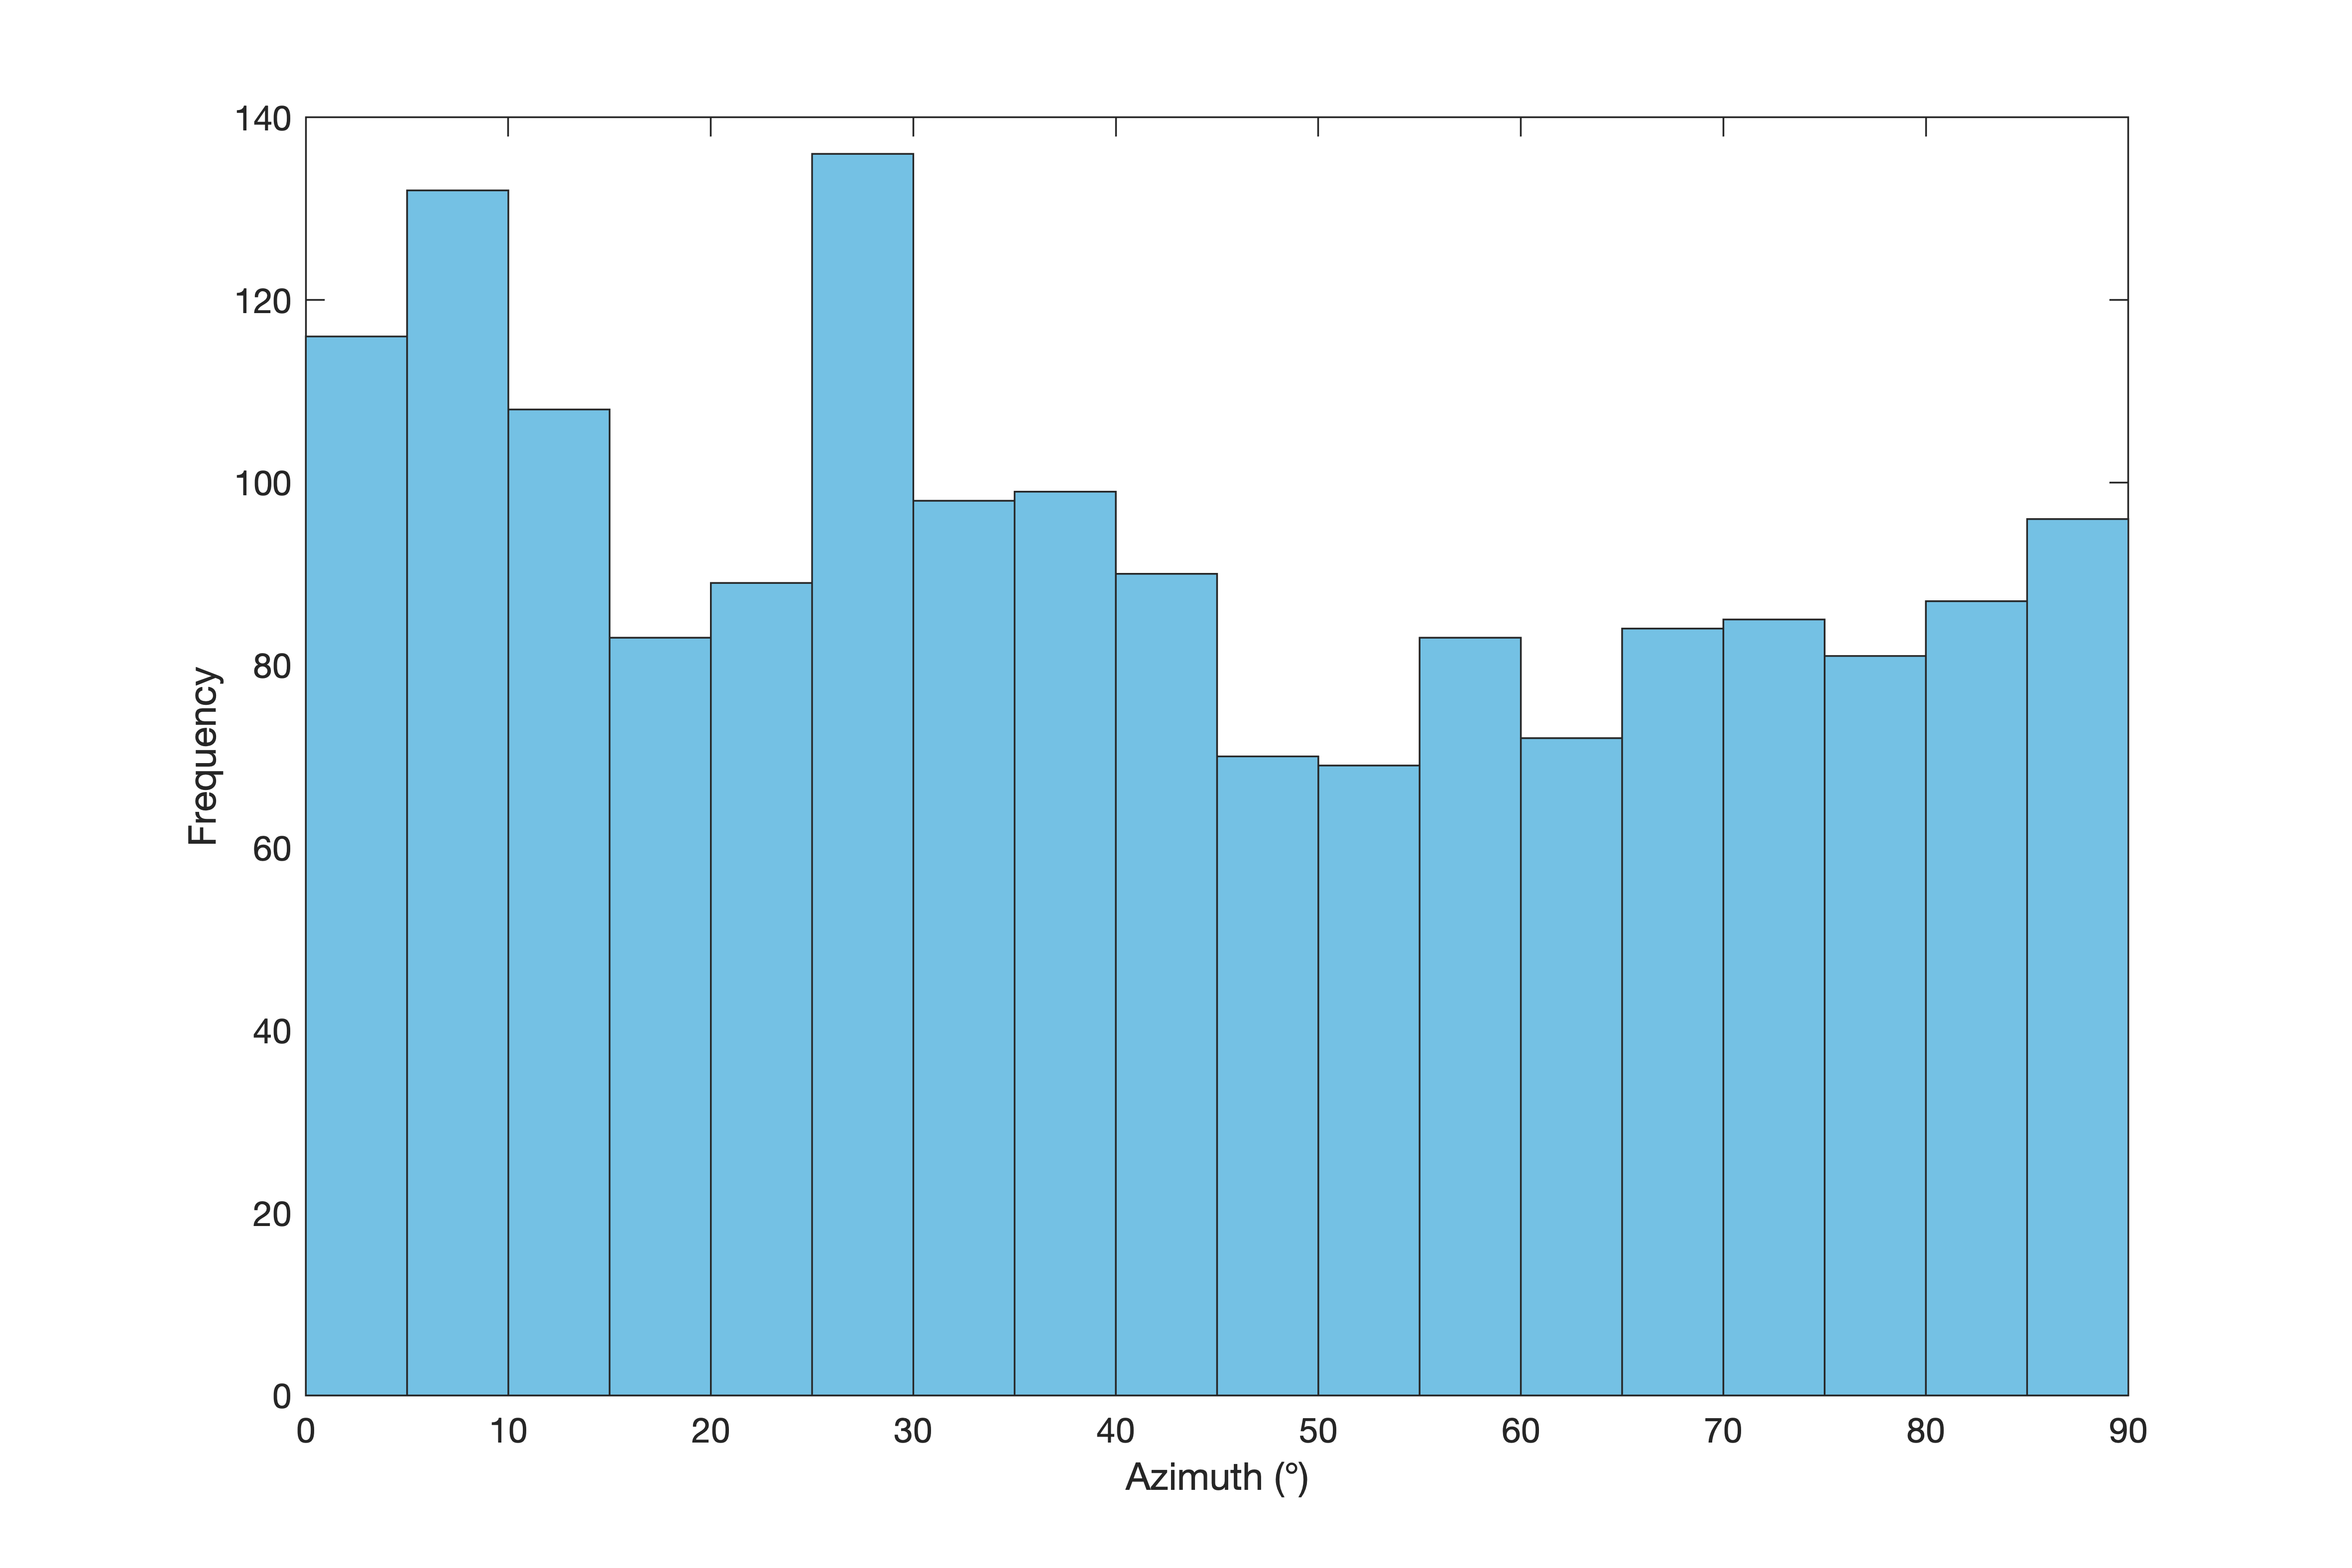
\includegraphics[width=\textwidth]{figures/fig4_4.png}
    \caption[Azimuth frequency histogram of traced craters]{Frequency histogram of number of elliptic craters traced per 5° azimuth bin for both the lAv and AHv units.}
    \label{fig:4-4}
\end{figure}

\chapter{Conclusion}
\label{chapter:5}

Given that Mars obliquity oscillates chaotically over >100~Ma time scales, constraining its historical path requires the careful use of statistical analysis and geologic evidence. Using the impact cratering forward-model developed by \citet{holo2018a}, and gathering fresh geologic evidence in the form of 1,678 elliptic crater traces on two geologic units of different ages (the lAv unit and AHv unit), we attempted to constrain the mean obliquity of Mars over the past $\sim$0.9~Ga and the past $\sim$2.0~Ga, finding that they were 66° (56.2°--74.6° standard deviation interval) and 8° (0.0°--14.4° standard deviation interval) respectively. Our procedure comprised first generating azimuth distributions of simulated craters under different obliquity scenarios, then normalizing those craters for the relevant latitude distributions associated with the sampled areas, and finally performing $\chi^2$ tests to measure the extent of mismatch between the simulated data from each obliquity scenario and the real observations. This result, if correct, implies that Mars, during its high-obliquity recent (past $\sim$0.9~Ga) past, saw greater water-ice sublimation, water-ice migration to the middle- and low latitudes, higher water vapor pressure, and more frequent polar dust storms; and, during its low-obliquity further (past $\sim$2.0~Ga) past, saw extensive polar glaciation, polar atmospheric collapse, and deep aquifer desiccation.

Our interpretation of these results considers several factors. First, our results are only partially congruent with those of \citet{holo2018a}. On the one hand, the low mean obliquity over the past $\sim$2.0~Ga is compatible with their mean obliquity estimate for the past $\sim$3.5~Ga, between $\sim$10° and $\sim$30°. On the other hand, however, the fraction of time spent at high obliquity, per this study’s results, most likely exceeds the one-fifth estimate. Second, implementing a procedure that considers inter-analyst error moderates the mean obliquity estimates to (in our median result) 63° (54.7°--72.0° standard deviation interval) and 14° (6.3°--20.5° standard deviation interval), respectively, and is likely required for our results to be internally compatible. Third, various limitations including the small number of elliptic craters, failure to check for poke-through older craters and caveats about \citet{holo2018a}’s pipeline require that further investigation continue to probe the past obliquity of Mars. Further research can continue with the present method by amassing a more comprehensive set of craters and quantifying the errors caused by poke-throughs of older craters on younger terrain. Adopting a more critical lens, future work should cross-check this study’s methods with \citet{holo2018a}’s by applying it to \citet{holo2018a}’s dataset and vice versa and re-evaluate the study’s unphysical result for the intervening $\sim$1.06~Ga period between the ages of the units.

% Format a LaTeX bibliography
\bibliographystyle{apa-good}
\makebibliography
\nocite{*}

\chapter*{Appendix: Code}
\addcontentsline{toc}{chapter}{Appendix: Code}

\section*{A.1\ \ \ \texttt{hu\_01\_get\_crater\_data.m}}
\addcontentsline{toc}{section}{A.1\ \ \ \texttt{hu\_01\_get\_crater\_data.m}}
\inputminted{matlab}{code/hu_01_get_crater_data.m}

\section*{A.2\ \ \ \texttt{hu\_02\_get\_azimuth\_diffs.m}}
\addcontentsline{toc}{section}{A.2\ \ \ \texttt{hu\_02\_get\_azimuth\_diffs.m}}
\inputminted{matlab}{code/hu_02_get_azimuth_diffs.m}

\section*{A.3\ \ \ \texttt{hu\_03\_get\_pois.m}}
\addcontentsline{toc}{section}{A.3\ \ \ \texttt{hu\_03\_get\_pois.m}}
\inputminted{matlab}{code/hu_03_get_pois.m}

\section*{A.4\ \ \ \texttt{hu\_04\_apply\_obliquity.m}}
\addcontentsline{toc}{section}{A.4\ \ \ \texttt{hu\_04\_apply\_obliquity.m}}
\inputminted{matlab}{code/hu_04_apply_obliquity.m}

\section*{A.5\ \ \ \texttt{hu\_05\_apply\_lat\_dist.m}}
\addcontentsline{toc}{section}{A.5\ \ \ \texttt{hu\_05\_apply\_lat\_dist.m}}
\inputminted{matlab}{code/hu_05_apply_lat_dist.m}
\inputminted{matlab}{code/hu_05a_find_lat_dist.m}

\section*{A.6\ \ \ \texttt{hu\_06\_get\_mismatch.m}}
\addcontentsline{toc}{section}{A.6\ \ \ \texttt{hu\_06\_get\_mismatch.m}}
\inputminted{matlab}{code/hu_06_get_mismatch.m}
\inputminted{matlab}{code/hu_06a_chi2test.m}
\inputminted{matlab}{code/hu_06b_gaussamp.m}

\section*{A.7\ \ \ \texttt{hu\_07\_plot\_age\_obliquity.m}}
\addcontentsline{toc}{section}{A.7\ \ \ \texttt{hu\_07\_plot\_age\_obliquity.m}}
\inputminted{matlab}{code/hu_07_plot_age_obliquity.m}

\section*{A.8\ \ \ \texttt{hu\_08\_perturb\_data\_iaerr.m}}
\addcontentsline{toc}{section}{A.8\ \ \ \texttt{hu\_08\_perturb\_data\_iaerr.m}}
\inputminted{matlab}{code/hu_08_perturb_data_iaerr.m}

\section*{A.9\ \ \ \texttt{hu\_09\_get\_mismatch\_var\_ecrit.m}}
\addcontentsline{toc}{section}{A.9\ \ \ \texttt{hu\_09\_get\_mismatch\_var\_ecrit.m}}
\inputminted{matlab}{code/hu_09_get_mismatch_var_ecrit.m}

\section*{A.10\ \,\texttt{hu\_10\_plot\_distributions.m}}
\addcontentsline{toc}{section}{A.10\ \,\texttt{hu\_10\_plot\_distributions.m}}
\inputminted{matlab}{code/hu_10_plot_distributions.m}

\end{document}